\documentclass[a4paper,man,natbib]{apa6}

\usepackage[english]{babel}
\usepackage[utf8x]{inputenc}
\usepackage{graphicx}
\usepackage{graphics}
\usepackage[colorinlistoftodos]{todonotes}
\usepackage{amsmath,amsfonts,mathabx}
\usepackage{epigraph}
\usepackage[figuresright]{rotating}
%\usepackage[ansinew]{inputenc}
\usepackage{multirow}
\usepackage{nameref}
%\setmainfont{Times New Roman} 
%\setsansfont{Times New Roman} 
%\setmonofont{Times New Roman} 
% Keywords command

\newcommand{\cmmnt}[1]{\ignorespaces}

\providecommand{\keywords}[1]
{
  \textbf{\textit{Keywords---}} #1
}
\usepackage[doublespacing]{setspace}

\setlength\epigraphwidth{.8\textwidth}

\title{The Discrete Metric in Categorization Under Time Pressure}
% Effect of Time Pressure on Distance Metrics in Categorization
\shorttitle{Discrete Metric Under Time Pressure}
\author{Florian I. Seitz}
\affiliation{University of Basel}

\abstract{The generalized context model \citep{nosofsky1986attention}, which excels at explaining human categorization behavior, assumes the Minkowski metric to represent psychological distance. I propose that in categorization under time pressure people compare stimuli heuristically with the discrete metric which counts the number of non--identical feature values for a given stimulus pair. 
61 psychology students from the University of Basel took part in a categorization experiment that manipulated the existence of time pressure between--subjects. Participants first learned without time pressure the category membership of eight stimuli under trial--by--trial supervision. Then, participants categorized six novel and four old stimuli 14 times without feedback in the test phase. Time pressure was applied to a random half of participants in the test phase.
%61 psychology students from the University of Basel acquired the category structure of eight stimuli with three four--valued features  in the learning phase under trial--by--trial supervision. After meeting the accuracy criterion participants categorized six novel and four old stimuli 14 times without feedback in the test phase. We applied time pressure to a random half of participants in the test phase.
Inferential tests at the aggregate level showed that the model version with the Minkowski metric accounted for participants' categorization behavior both with and without time pressure ($p$ < .001, respectively). Computational cognitive modeling yielded that, without time pressure, the model with the discrete metric and attention on all features and, with time pressure, a random choice model outperformed the other models both on the aggregate and on the individual level.
The present findings suggest that under time pressure, people don't use the discrete metric. These findings imply that higher cognitive load doesn't reduce the complexity of psychological distance computation in categorization, but rather increases choice inconsistency. 
%We discuss related literature on choice inconsistency in preferential choice and also discuss to what extent a rule--based model could account for our findings.
} 

\keywords{categorization, time pressure, Minkowski metric, discrete metric, psychological distance}

\begin{document}
\maketitle

%\vspace*{\fill}
\epigraph{There is nothing more basic than categorization to our thought, perception, action, and speech. [...] An understanding of how we categorize is central to any understanding of how we think and how we function, and therefore central to an understanding of what makes us human.}{George Lakoff, 1987, pp.5--6}

Humans frequently engage and excel in categorization---the generation and identification of groups from a bigger amount of objects. Categorization is thus considered one of the most fundamental cognitive phenomena overall \citep{ashby2001categorization, bruner1956study, cohen2005bridging, lakoff1987women, goldstone2003concepts}. Past research has shed much light on the cognitive processes during categorization learning and generalization \citep[for an overview over the diverse cognitive models of categorization, see][]{kruschke2008models,wills2013models}. One finding from these studies is that people first rely on simple categorization strategies and only if necessary pass on to more complex strategies \citep{gluck2002people, meeter2006strategies, meeter2008probabilistic, johansen2002there, smith1998prototypes}. Simple categorization processes include the reduction of the number of attended features (resulting in an extreme case in a unidimensional classification process where categorization behavior depends only on one single feature ; \citealp{johansen2002there}) and by the use of a central tendency (i.e., a prototype) instead of multiple actual instances to represent a category \citep{smith1998prototypes}. 
%Both unidimensional strategies and prototype--based strategies have been found to account for human behavior during early categorization when people rely on simple strategies \citep{johansen2002there, smith1998prototypes}.

While unidimensional strategies and prototype--based strategies reduce the amount of information that enters the categorization process, another, remarkably different way to simplify the categorization process lies in simplifying the computation itself. This kind of simplification is the focus of the current study: Within the framework of the generalized context model \citep{nosofsky1986attention}, which bases the classification of an object on its similarity to category instances, I investigate a heuristic at the level of the psychological similarity function.
More specifically, I examine a computationally simple object comparison that checks the identity of two objects' values on a given feature and thus leads to binary feature differences. The computationally simple categorization process bases psychological similarity on these binary feature differences, whereas the more extensive categorization process base psychological similarity on metric feature differences. The present thesis tests this hypothesis in a categorization task under time pressure with an experimental design that optimally discriminates between the metric and binary difference computation while allowing as well to test the alternative strategy simplification of unidimensional strategies. 
%All strategies are implemented in the popular generalized context model \citep{nosofsky1984choice, nosofsky1986attention, nosofsky2011generalized} which is an exemplar--based model, where people retrieve instances from memory (i.e., exemplars) and compare them with an instance to categorize (i.e., the probe) to assess category membership \citep{medin1978context}. 

%Strategy simplification, however, has not been central in research on categorization under time pressure, albeit that in lack of time the need for simplifying the categorization process might be particularly pronounced. In contrast, research on the temporal aspects of categorization has focused on sequential information sampling such as competing retrieval of comparison objects from memory \citep{nosofsky1997exemplar, nosofsky1999effects, nosofsky2005speeded} or sequential processing of features (\citealp{lamberts1995categorization, lamberts1998time, lamberts2000information}; for a combination of both processes, see \citealp{cohen2003extension}). 

\subsection{Theoretical Background: Categorization under Time Pressure}
Categorizations often have to be carried out quickly. Imagine an emergency medical physician who has to quickly make a diagnosis in order to provide her patient with the right treatment or a traveler in the woods who has to decide whether a long, brown, and slightly curved object is a dangerous snake or a harmless branch. Fast categorization is required in both situations in order to prevent a negative outcome that results from delayed reaction. Empirical research, however, has only little investigated how people categorize objects under time pressure. 

One line of research attempts to uncover the temporal development of the categorization process \citep{lamberts2000information, lamberts2002feature, nosofsky1997exemplar}. Studies from this research line analyzed people's response times in perceptual categorization and modeled how people sequentially include information and adapt their categorization probabilities. One model that arose in this research is the exemplar--based random--walk model \citep{nosofsky1997exemplar} which assumes a sequential retrieval of exemplars from memory. Specifically, the exemplars race against each other for comparison with the probe. The similarity between the probe and every exemplars than won the race is computed and category membership probability is updated accordingly. Once a benchmark in favor of one of the categories is passed, people are assumed to render their response. Response times are hence dependent on the speed with which the different exemplars race, which is in turn a function of the exemplar's presentation frequency, presentation recency, and similarity to the probe. A second model of the temporal development is the extended generalized context model for response times \citep{lamberts2000information, lamberts2002feature} which assumes that people sequentially process the probe's features and thus serially construct a representation of the probe. The processed features of the probe are compared to the corresponding features of all stored exemplars in memory. The extended generalized context model for response times predicts response times to be dependent on how much stimulus information needs to be sampled until a categorization response can be rendered with sufficient confidence.

Both these approaches thus model response times by means of sequential information sampling and don't focus on the effect of response deadlines on categorization. However, the models' assumptions may be applied to categorization under time pressure and, in fact, the extended generalized context model for response times is derived from the extended generalized context model \citep{lamberts1995categorization}, which addresses just this topic. Assuming the same principle of sequential sampling of stimulus information, the extended generalized context model was shown to account for categorization under time pressure in a series of studies \citep{lamberts1995categorization, lamberts1998time, lamberts1999building, lamberts1999categorization, lamberts1997fast}. 
The majority of these studies analyzed the effect of time pressure on categorization in binary environments (i.e., where each feature contains only two possible values; \citealp{lamberts1995categorization, lamberts1998time, lamberts1999building, lamberts1999categorization}). In such binary environments, feature comparisons between stimuli cannot be simplified as two stimuli can differ on a given feature by maximally 1, which is the smallest amount of differences possible in order for a feature to contain any relevant information. The results from these studies are hence uninformative for the research question of this thesis, namely, whether people under time pressure simplify stimulus feature comparison. 

One study \citep{lamberts1997fast}, however, used stimuli with multivalued features and found that the extended generalized context model can account for categorization behavior in two experiments with time limits of 400 ms and 700 ms per trial. An alternative explanation to the findings of \cite{lamberts1995categorization} might be that participants simplify the feature comparisons between probe and exemplars when they face time pressure. Specifically, people may not compute metric feature differences between probe and exemplars under time pressure, but rely on a simple binary feature comparison which only checks for identity on a given feature. The metric feature comparison between probe and exemplars may be implemented by the Minkowski distance (see below for a formal description) which is, to my knowledge, the only measure of distance used in categorization models. The heuristic feature comparison that checks for identity of feature values is formalized by the discrete distance (see below for a formal description) and might replace the Minkowski metric in categorization under time pressure. In what follows, I will describe one of the most prominent models of categorization---the generalized context model \citep{nosofsky1986attention}---which assumes the Minkowski distance for comparisons between probe and exemplars and present an alternative version of the model that uses the discrete distance instead.

\subsection{Formal Models: The Generalized Context Model With two Distance Metrics}
One of the most prominent formal models for human categorization is the generalized context model \citep{nosofsky1984choice, nosofsky1986attention, nosofsky2011generalized} which is an exemplar--based model, where people retrieve instances from memory (i.e., exemplars) and compare them with an instance to categorize \citep[i.e., the probe;][]{medin1978context}. People are assumed to represent each exemplar as a point in a multidimensional space where the exemplar's feature values are the point's coordinates. Comparisons between probe and exemplars are expressed as distances, which can be interpreted as how far away the probe is spatially positioned from the exemplar of comparison. Distances are transformed into similarities, such that high distances correspond to low similarities and low distances to high similarities. Finally, the aggregate similarity of the probe to all exemplars of one category relative to the aggregate similarity to all exemplars states the model's prediction of category membership for the probe. The higher the similarity of the probe to the exemplars of one category the higher the model's prediction of assigning the probe into this very category. 

In the following, I will describe the three computational steps of distance, similarity, and categorization probability which the generalized context model assumes in a multidimensional, multivalued stimulus space with two categories. The formalization of the model is equivalent to \cite[][pp.281--282]{nosofsky1989further}, except that it has been generalized to more than two dimensions. 

\subsubsection{Categorization probability}
The generalized context model \citep{nosofsky1989further} predicts a probe's category membership by means of the similarity between the probe and the categories to choose from. Specifically, the probability with which probe $i$ is categorized into category $A$ is defined as 
\begin{equation}
P(R_{A}|i) = \frac{b_{A}\sum\limits_{j \in A} s_{ij}}{b_{A}\sum\limits_{j \in A} s_{ij} + (1 - b_{A})\sum\limits_{k \in B} s_{ik}},
\label{eq:probability}
\end{equation}
where $P(R_{A}|i)$ is the probability of assigning probe $i$ to category $A$, $s_{ij}$ is the similarity between probe $i$ and exemplar $j$, and $b_{A}$ is the response bias for category $A$ (with $0 \leq b_{A} \leq 1$). The function assumes probabilistic categorization in accordance with the relative aggregate similarity that is attributable to one of the two categories. The function is often referred to as Luce's choice axiom \citep{luce1959individual} and is derived from the similarity--choice model for stimulus identification \citep{luce1963detection, shepard1957stimulus}. 

\subsubsection{Similarity}
The similarity $s_{ij}$ between probe $i$ and exemplar $j$, which is needed for categorization probability, is itself computed from the distance between $i$ and $j$ in a multidimensional space. The transformation of distance into similarity is given by Shepard's universal law of generalization \citep{shepard1987toward}
\begin{equation}
s_{ij} = \exp\left(-c*d_{ij}^p\right),
\label{eq:similarity}
\end{equation}
where $d_{ij}$ is the distance between probe $i$ and exemplar $j$, $c$ (with $0 \leq c$) is an overall sensitivity parameter, and $p$ is a parameter that determines how similarity relates to psychological distance. Popular versions of the similarity function are the exponential decay function ($p = 1$) for discriminable stimuli and the Gaussian function ($p = 2$) for confusable stimuli \citep{ennis1988confusable, nosofsky1985luce}. The sensitivity parameter $c$ describes the convexity of the similarity function indicating thus the steepness with which similarity decreases at small distances. For high values of $c$, similarities are already low at small distances. For low values of $c$, similarities are still high at large distances. In both cases, the model only weakly discriminates between different sizes of distance. The parameter $c$ thus denotes a person's sensitivity to psychological distance.

\subsubsection{Distance}
As a requisite to assess the similarity, the generalized context model computes distances between probe and exemplars in a multidimensional space. A vast number of distance metrics exist that could represent the psychological distance of two objects \citep{deza2009encyclopedia}. In fact, the only prerequisites that geometric distance metrics need to meet are (a) the non--negativity axiom (all distances are greater than or equal to 0), (b) the identity of indiscernibles (distances between identical objects are 0), (c) symmetry (the distance between two objects is independent of the order of the objects), and (d) the triangle inequality (the distance between two objects is at least as small as the distance of these two objects via a third object; \citealp{restle1959metric}). The generalized context model and related models of categorization assume the Minkowski distance. I propose that under time pressure people use the discrete distance.

\paragraph{Minkowski distance}
The Minkowski distance is formally implemented in the generalized context model as
\begin{equation}
d_{ij} = \left[\sum\limits_{m=1}^M w_{m}*\mid x_{im} - x_{jm}\mid ^r\right]^\frac{1}{r},
\end{equation}
where $d_{ij}$ is the distance between probe $i$ and exemplar $j$, $x_{im}$ is the value of probe $i$ on feature $m$, $w_{m}$ is the attention weight attributed to feature $m$ (with $0 \leq w_{m} \leq 1$ and $\sum w_{m} = 1$ \footnote{Note that the attention weights $w$s are a psychological extension of the Minkowski metric that represent differential allocation of attention across features. In its mathematical definition the Minkowski distance doesn't include attention weights.}), $M$ is the number of features, and $r$ describes the form of the distance metric (with $r \geq 1$). Popular instances of the Minkowski distance are the Manhattan distance ($r = 1$) for highly separable features and the Euclidean distance ($r = 2$) for integral features \citep{shepard1964attention, nosofsky1986attention, garner1974processing}. Values of $r$ are constrained to be equal to or higher than 1 for adherence with the triangle inequality \citep{jakel2008similarity,francois2007concentration,tversky1982similarity,beals1968foundations}. For $r < 1$ the Minkowski distance between probe $i$ and exemplar $j$ may thus be larger than the summed Minkowski distance between probe $i$ and exemplar $k$ and between exemplar $k$ and exemplar $j$ and in such a case the Minkowski distance is not anymore a metric \citep[][p. 5]{kress1989linear}. 

\paragraph{Discrete distance}
The discrete distance is formally given by 
\begin{equation}
d_{ij} = \left[\sum\limits_{m=1}^M w_{m}* \rho_{m}(x_{im}, x_{jm}) ^r\right]^\frac{1}{r},
\label{eq:distance}
\end{equation}

where $\rho_{m}(x_{im}, x_{jm})$ is the discrete distance function that checks whether probe $i$ and exemplar $j$ have an identical value on dimension $m$. Checking the identity of feature values can result in a distance of 1, if probe $i$ and exemplar $j$ are not identical on dimension $m$, or in a distance of 0, if they are identical. In the generalized context model, this yields

\begin{equation}
\rho_{m}(x_{im}, x_{jm}) = 
\begin{cases}
	1 & x_{im} \neq x_{jm} \\
	0 & else 
\end{cases}.
\end{equation}

All parameters of the generalized context model are preserved in the version with the discrete distance; the only difference to the model version with the Minkowski metric lies in the way how distances between objects are computed.

\subsubsection{Relation to the unidimensional generalized context model}
Instead of using the heuristical discrete metric to simplify categorization under time pressure, people might as well base their categorization behavior on fewer stimulus features. In an extreme case, participants only attend to one feature, probably the feature they deem most relevant, and categorize a probe only based on this single feature. In the generalized context model \citep{nosofsky1989further} attention partition across features is given by the attention weights $w$s. Whereas in the multidimensional generalized context model attention weights are only constrained to be positive and to sum up to 1, in the unidimensional generalized context model one of the attention weights is set to 1 and the remaining to 0. In a given environment, there exist as many unidimensional generalized context model versions as the stimuli contain features. An important distinction between the unidimensional and the multidimensional generalized context model is that the unidimensional model version cannot model feature interactions. 

In the present study, people had to learn a non--linearly separable category structure which requires people to attend to multiple features. In other words, the unidimensional generalized context model cannot learn the category structure of the present study. As the unidimensional generalized context model fails to reach sufficient categorization accuracy during learning, I hypothesize that people under time pressure lower their computational load by means of a simple psychological distance computation (i.e., the discrete metric) instead of using the unidimensional generalized context model. The present thesis also investigates the unidimensional generalized context model with the discrete metric which needs the least computational power as both the distance metric is simplified and less features are attended to. In case this model describes a participant this is counted as evidence for the discrete metric as the primary aim of this thesis is to analyze whether people use different distance metrics depending on the amount of cognitive load.
%in conditions with time pressure and without time pressure.
 
\subsubsection{Relation to prototype models}
Whereas the generalized context model bases categorization on the similarity between probe and exemplars (i.e., actual instances experienced in the past; \citealp{medin1978context, nosofsky1986attention}), prototype models base categorization on the similarity between probe and prototypes (i.e., abstract central tendencies; \citealp{posner1968genesis}). Hence, in comparison to the generalized context model, prototype models cannot depict influences from individual exemplars directly, but only indirectly via prototypes \citep{nosofsky2011generalized, nosofsky1992exemplars, medin1978context}.
% Due to the very fine--grained representation of categories using actual experienced instances, the categorization predictions of the generalized context model are sensitive to influences from individual exemplars---influences which are absent in prototype models \citep{nosofsky2011generalized, nosofsky1992exemplars, medin1978context}. 
%Following a long debate of whether people represent categories using prototypes or exemplars, research indicates that exemplar-based categorization models using a non--linear similarity rule, such as the generalized context model, outperform prototype models in explaining participants' categorization behavior (\citealp{nosofsky1992exemplars}, see also \citealp{scholkopf2002learning}). However, further evidence indicates that people shift from a prototype--based model during early categorization to a computationally more complex exemplar--based model as the number of experienced exemplars increases (\citealp{smith1998prototypes}, but for an alternative view, see \citealp{nosofsky2002exemplar}). 

On the computational level, prototype models require people to abstract a central tendency of a category. In turn, people don't have to retrieve the individual exemplars of the category and thus have to process less information during categorization. Prototype models depict thus a computationally simple categorization process that considers only summary category information.
Still, I didn't integrate a prototype--based model in the present thesis, as design optimization revealed that no design simultaneously may recover and discriminate the two distance metrics (i.e., the Minkowski and the discrete metric) and the two types of category representation (i.e., prototypes and exemplars). Furthermore, in the present study, participants had to learn the category membership of only a few stimuli in a non--linearly separable category structure---two design properties for which literature suggests that people use exemplar--based strategies \citep{smith1998prototypes, smith2000thirty}. Hence, I assume for the categorization task of the present study that people use an exemplar--based model, namely the well--established generalized context model \citep{nosofsky1986attention}.

\subsection{Hypotheses}
The present thesis investigates whether psychological distance is computed heuristically in categorization with limited cognitive resources. Psychological distance is operationalized in the present study within the framework of the generalized context model \citep{nosofsky1989further} with two different distance metrics---the Minkowski metric and the heuristic discrete metric. Allowing both model versions of the generalized context model to attend to several features (i.e., multidimensional model versions) or to only one feature (i.e., unidimensional model versions) further enables to examine the amount of stimulus information processed in categorization with limited cognitive resources. In the present study, limited cognitive resources are operationalized with time pressure, as time is a fundamental cognitive resource in decision--making. In the baseline condition without time pressure, I expect people to use the well--established multidimensional Minkowski metric; in the condition with time pressure I expect people to use the heuristic discrete metric (either unidimensional or multidimensional). Based on this main hypothesis, I state the following specific hypotheses which all presuppose the use of the generalized context model: 

Under time pressure, people use the discrete metric (H1a), else a unidimensional Minkowski metric (H1b), else the multidimensional Minkowski metric (H1c). Across participants, the multidimensional and the unidimensional discrete metric outperform the remaining models in predicting participant behavior, followed by the unidimensional Minkowski metric on the second rank, the multidimensional Minkowski metric on the third rank, and the random choice model on the final rank (H1d). At the individual level, the multidimensional and the unidimensional discrete metric describe more participants than any of the remaining models (H1e). Furthermore, at the individual level, the rank order of H1d is found as well in the count of participants best described by each model (H1f). 

Without time pressure, people use the multidimensional Minkowski metric (H2a). Across participants, the multidimensional Minkowski metric outperforms the remaining models, while the random choice model is inferior to all remaining models in predicting participant behavior (H2b). I have no hypotheses about the relative performance amongst the unidimensional Minkowski metric, the unidimensional discrete metric, and the multidimensional discrete metric. At the individual level, the multidimensional Minkowski metric describes more participants than any of the remaining models and the rank order of H2b is as well found in the count of participants best described by each model (H2c). 

Finally, the multidimensional discrete metric describe more participants with time pressure than without time pressure (H3a), whereas the multidimensional Minkowski metric describes more participants without time pressure than with time pressure (H3b).

\section{Method}

\subsection{Optimal Experimental Design}
I designed the experimental task using optimal experimental design \citep{myung2009optimal}. An optimal experimental design is defined as a design with ``the greatest likelihood of differentiating the models under consideration'' \cite[][p. 500]{myung2009optimal}. Being able to discriminate between the discrete metric and the Minkowski metric means that each model is associated with unique expected behavioral predictions in the experimental design. The models under consideration can thus be discriminated well by the data, in the expectation. Furthermore, through the maximization of model prediction differences, design optimization increases model recovery (i.e., the best--fitting model is also the model underlying the data; however, each scientific model is only an approximation of the participant's cognitive model, see \citealp{myung2009optimal}). The advantages of design optimization are thus two-fold: A participant's behavior can be associated more exclusively with one of the models under consideration and, given that the participant used one of the models under consideration, the probability is higher that this best--fitting model is the data--generating model. Design optimization maximizes thus the experiment's degree of informativeness and cost-effectiveness while keeping the necessary sample and trial size at a low level \citep{cavagnaro2009better, ouyang2016practical, raffert2012optimally, atkinson2007optimum, nelson2005finding}. 

The advantages of design optimization are most pronounced when the different models differ quantitatively instead of qualitatively as well as when several variables have to be considered simultaneously during the designing process of the experiment making thus a good design hardly visible to the naked eye \citep{myung2009optimal}. Both criteria apply to the present study.
The potential of optimal experimental design is shown in a reanalysis of the designs of the first two experiments of \cite{smith1998prototypes} which aimed at distinguishing the generalized context model \citep{nosofsky1986attention} from the multiplicative prototype model \citep{smith1998prototypes} by using six--dimensional binary stimuli \citep{myung2009optimal}. Even though the best experimental design used in \citeauthor{smith1998prototypes} had a high model recovery of 88.8\%, the optimal design that was possible yielded a model recovery rate of 96.3\%, minimizing thus the risk of a model fitting error by eight percent.  

In light of these insights, I ran simulations to find a categorization environment such that the discrete metric and the Minkowski metric implemented in the generalized context model can be optimally discriminated given the responses during the test phase, in the expectation.\footnote{In the first simulations we further wanted to discriminate the generalized context model from the multiplicative prototype model. However, as simultaneously discriminating the two models and the two distance metrics led to insufficient model recovery rates, we dropped the multiplicative prototype model from the remaining simulation analyses.} The simulations were chronologically iterated over (a) the design (i.e., all possible category structures with equal category base rates for all subsets of eight of 64 stimuli in the learning phase, under the constraint that learning stimuli differ from each other maximally by 1 unit per feature to ensure that the discrete and the Minkowski metric yield identical distances and thus none is favored by the learning phase design), (b) the true model (i.e., the generalized context model with either the Minkowski metric or the discrete metric), (c) the true parameter combination (i.e., attention weights $w$'s ranging from $0$ to $1$ in steps of $1/3$ and the overall sensitivity parameter $c$ ranging from $0.1$ to $4.1$ in steps of $1$), and (d) the fitting model (i.e., the generalized context model with either the Minkowski metric or the discrete metric).

For a given design, true model, and true parameter combination we simulated binary participant responses (i.e., category A or B) based on the true model's predictions for the learning set which was replicated 20 times and for the test set (i.e., the stimuli that were not part of the learning stimuli) which was replicated 10 times. Then, the free parameters (i.e., attention weights $w$s and the overall sensitivity parameter $c$) of both models were fit to the simulated data of the learning set excluding the first eight trials and fixed to the resulting optimal parameters for each participant. Next, predictions for the test set were computed with both fitted models and the log likelihood between the simulated participant responses under the true model and the predictions of each fitted model was calculated for the test phase data. This procedure allowed conducting model recoveries for every design across all permissible parameter combinations. The optimal design was the design for which the winning model recovered the true data--simulating model best across the permissible model parameters. In the optimal design, the learning criterion was met by both models when adding a softmax choice rule. From the 56 stimuli in the test phase of the best design, the six stimuli that discriminated models best were selected. Figure \ref{fig:environment} shows the stimuli in the resulting design.

\subsection{Materials and Design}
The experiment was conducted on \textit{computers; I need to describe them in more detail} and programmed in Expyriment \citep{krause2014expyriment} based on prior work by \cite{albrechtxxxunstacking}. Participants classified different stimuli into two categories by pressing the left and right arrow keys. The stimuli were based on the material of \cite{albrechtxxxunstacking}. Each stimulus consisted of three features represented by grey beams with feature values ranging from one to four and being represented by colored squares. Figure \ref{fig:material} illustrates the material. Participants learned the category structure of eight stimuli in the learning phase, and categorized four of them and six novel stimuli in the test phase (see Figure \ref{fig:environment}). Table \ref{tab:environment} shows the median model predictions for all stimuli of the learning set and the test set. Category labels, the key--label association, the color--feature association, and the visual mapping of features to positions on the screen were randomized across participants.

\begin{figure}[htbp]
\centering
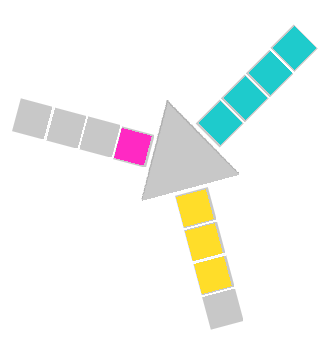
\includegraphics[width = \textwidth]{fig_material.PNG}
\caption{Products used as stimuli in the experiment. Each grey beam illustrates an ingredient (i.e., a feature) and the colored squares illustrate the number of quantity units for each ingredient (i.e., the feature value).}
\label{fig:material}
\end{figure}

\begin{figure}[htbp]
\centering
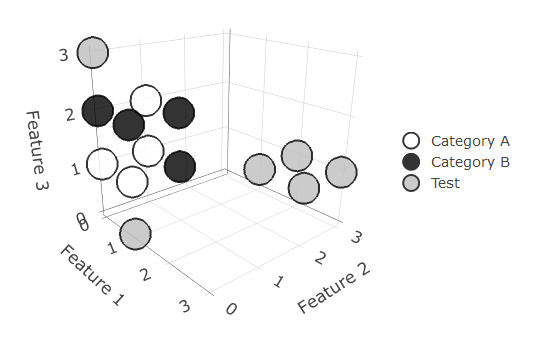
\includegraphics[width = \textwidth]{fig_environment.png}
\caption{Learning stimuli (in black and white) including their category membership and test stimuli (in grey). Each axis of the graph represents one feature, and the coordinates of each sphere represent the feature values of the respective stimulus. Stimuli in the learning phase include all learning stimuli, stimuli in the test phase include all test stimuli as well as the learning stimuli 002, 012, 101, and 111.}
\label{fig:environment}
\end{figure}

\begin{sidewaystable}
\begin{center}
\begin{threeparttable}
\caption{Environment used and median model predictions}
\label{tab:environment}
\begin{tabular}{cccccccccc}
\toprule
 &  & \multicolumn{4}{c}{Discrete} & \multicolumn{4}{c}{Minkowski} \\
\cmidrule(r){3-6} \cmidrule(r){7-10}
 &  & \multicolumn{1}{c}{Multidimensional} & \multicolumn{3}{c}{Unidimensional} & \multicolumn{1}{c}{Multidimensional} & \multicolumn{3}{c}{Unidimensional} \\
\cmidrule(r){4-6} \cmidrule(r){8-10}
Stimulus & \multicolumn{1}{c}{Category} &  & \multicolumn{1}{c}{$w$_1 = 1} & \multicolumn{1}{c}{$w$_2 = 1} & \multicolumn{1}{c}{$w$_3 = 1} &  & \multicolumn{1}{c}{$w$_1 = 1} & \multicolumn{1}{c}{$w$_2 = 1} & \multicolumn{1}{c}{$w$_3 = 1}\\
\midrule
\addlinespace
\multicolumn{2}{c}{\emph{Learning phase}} \\
\addlinespace
001 & B & 0.97 & 0.74 & 0.50 & 0.74 & 0.97 & 0.74 & 0.50 & 0.74\\
002\makebox[0pt][l]{$^{\ast}$} & A & 0.09 & 0.74 & 0.50 & 0.26 & 0.09 & 0.74 & 0.50 & 0.26\\
011 & B & 0.99 & 0.74 & 0.50 & 0.74 & 0.99 & 0.74 & 0.50 & 0.74\\
012\makebox[0pt][l]{$^{\ast}$} & B & 0.93 & 0.74 & 0.50 & 0.26 & 0.93 & 0.74 & 0.50 & 0.26\\
101\makebox[0pt][l]{$^{\ast}$} & B & 0.91 & 0.26 & 0.50 & 0.74 & 0.91 & 0.26 & 0.50 & 0.74\\
102 & A & 0.03 & 0.26 & 0.50 & 0.26 & 0.03 & 0.26 & 0.50 & 0.26\\
111\makebox[0pt][l]{$^{\ast}$} & A & 0.07 & 0.26 & 0.50 & 0.74 & 0.07 & 0.26 & 0.50 & 0.74\\
112 & A & 0.01 & 0.26 & 0.50 & 0.26 & 0.01 & 0.26 & 0.50 & 0.26\\
\midrule
\addlinespace
\multicolumn{2}{c}{\emph{Test phase}} \\
\addlinespace
003 & - & 0.63 & 0.74 & 0.50 & 0.50 & 0.09 & 0.74 & 0.50 & 0.26\\
100 & - & 0.37 & 0.26 & 0.50 & 0.50 & 0.91 & 0.26 & 0.50 & 0.74\\
221 & - & 0.85 & 0.50 & 0.50 & 0.74 & 0.07 & 0.26 & 0.50 & 0.74\\
231 & - & 0.85 & 0.50 & 0.50 & 0.74 & 0.07 & 0.26 & 0.50 & 0.74\\
321 & - & 0.85 & 0.50 & 0.50 & 0.74 & 0.07 & 0.26 & 0.50 & 0.74\\
331 & - & 0.85 & 0.50 & 0.50 & 0.74 & 0.07 & 0.26 & 0.50 & 0.74\\
\bottomrule
\addlinespace
\end{tabular}
\begin{tablenotes}[para]
\textit{Note.} Median model predictions for the stimuli used in the learning phase and the test phase. The four stimuli from the learning phase marked with an asterisk also appeared in the test phase.
\end{tablenotes}
\end{threeparttable}
\end{center}
\end{sidewaystable}

Participants' main task was to categorize stimuli into two categories. The stimuli were described to the participants as products and the two categories were operationalized as brands (i.e., brand L and brand R). The dependent variable was the categorization decision. The independent variable was the time pressure induced every second participant in the test phase. It allowed a participant 400 milliseconds plus 30\% of the median decision time needed by this participant across the final 100 learning trials. The study had thus a repeated--measures 2x1 between--subjects design. Further variables assessed were response times for each trial and the absolute time pressure if any.

\subsection{Participants}
Data was collected from \textit{start date} till \textit{end date}. Psychology students from the University of Basel were recruited over an online platform of the Faculty of Psychology to participate in a categorization study. All participants had a high--school or a higher degree and were asked about color blindness, visual impairment, and in case of impaired vision whether they carried a visual aid during the experiment. Participants selected themselves into the sample and there were no inclusion criteria. Up to six participants could show up to the same experimental session. As a compensation for study participation subjects received course credit proportionally to the amount of time needed to complete the study. Participant data were listwise deleted if (a) the participant failed to reach the accuracy criterion in the learning phase within an hour, (b) answered ''absolutely unclear'' or ''somewhat unclear'' to the question if the task in the experiment was clear or (c) in the time pressure condition exceeded the time limit in more than 50\% of the test trials for a given test stimulus and in the no time pressure condition had a log transformed reaction time more than three standard deviations below the mean of the log transformed reaction times of the learning phase in more than 50\% of the test trials for a given test stimulus. Out of 73 people who showed up, two did not complete the experiment as they didn't achieve the accuracy criterion within an hour. Two of the remaining 71 participants were used for pretest purposes and additional eight participants had to be excluded from analyses as they reported that the task was somewhat or absolutely unclear to them. No participant had to be excluded due to the reaction time criterion. This resulted in 61 participants (43 females, $M_{age}$ = 24.13 years, $SD_{age}$ = 6.39 years, age range: 19--50 years) used for statistics and data analysis, out of which 30 had time pressure in the test phase and 31 didn't.  

Sample size was predetermined by a model--based power simulation. Across participants the true probability of choosing the Minkowski metric changed from 70\% to 30\% and the true probability of choosing the discrete metric changed from 30\% to 70\% when time pressure was introduced. For every participant, a random combination of parameters that met the accuracy criterion was sampled for the two model versions, respectively, and a mixing probability was sampled from a normal distribution truncated between 0 and 1 with the mean being equal to the share of participants using the discrete metric in the respective time pressure condition and SD =  .3. For any given test phase trial the mixing probability indicated how much the predictions of the discrete model version influenced the probabilities underlying simulated participant responses relatively to the predictions of the Minkowski model version. The log likelihood of the simulated responses was calculated for both model versions on the participant level and transformed into Akaike weights \citep{wagenmakers2004aic}. A given model was accepted if its Akaike weight exceeded .95. One--sided two proportion z--tests were calculated for each sample size comparing the proportion of accepted discrete model versions with time pressure and without time pressure. Figure \ref{fig:power} illustrates the proportion of significant results for every sample sizes across 1000 iterations. Given an aspired power of .8, a total sample size of N = 60 (n = 30 in each condition) was necessary to achieve 89\% power. The final sample included 31 participants without time pressure and 30 participants with time pressure.

\begin{figure}[htbp]
\centering
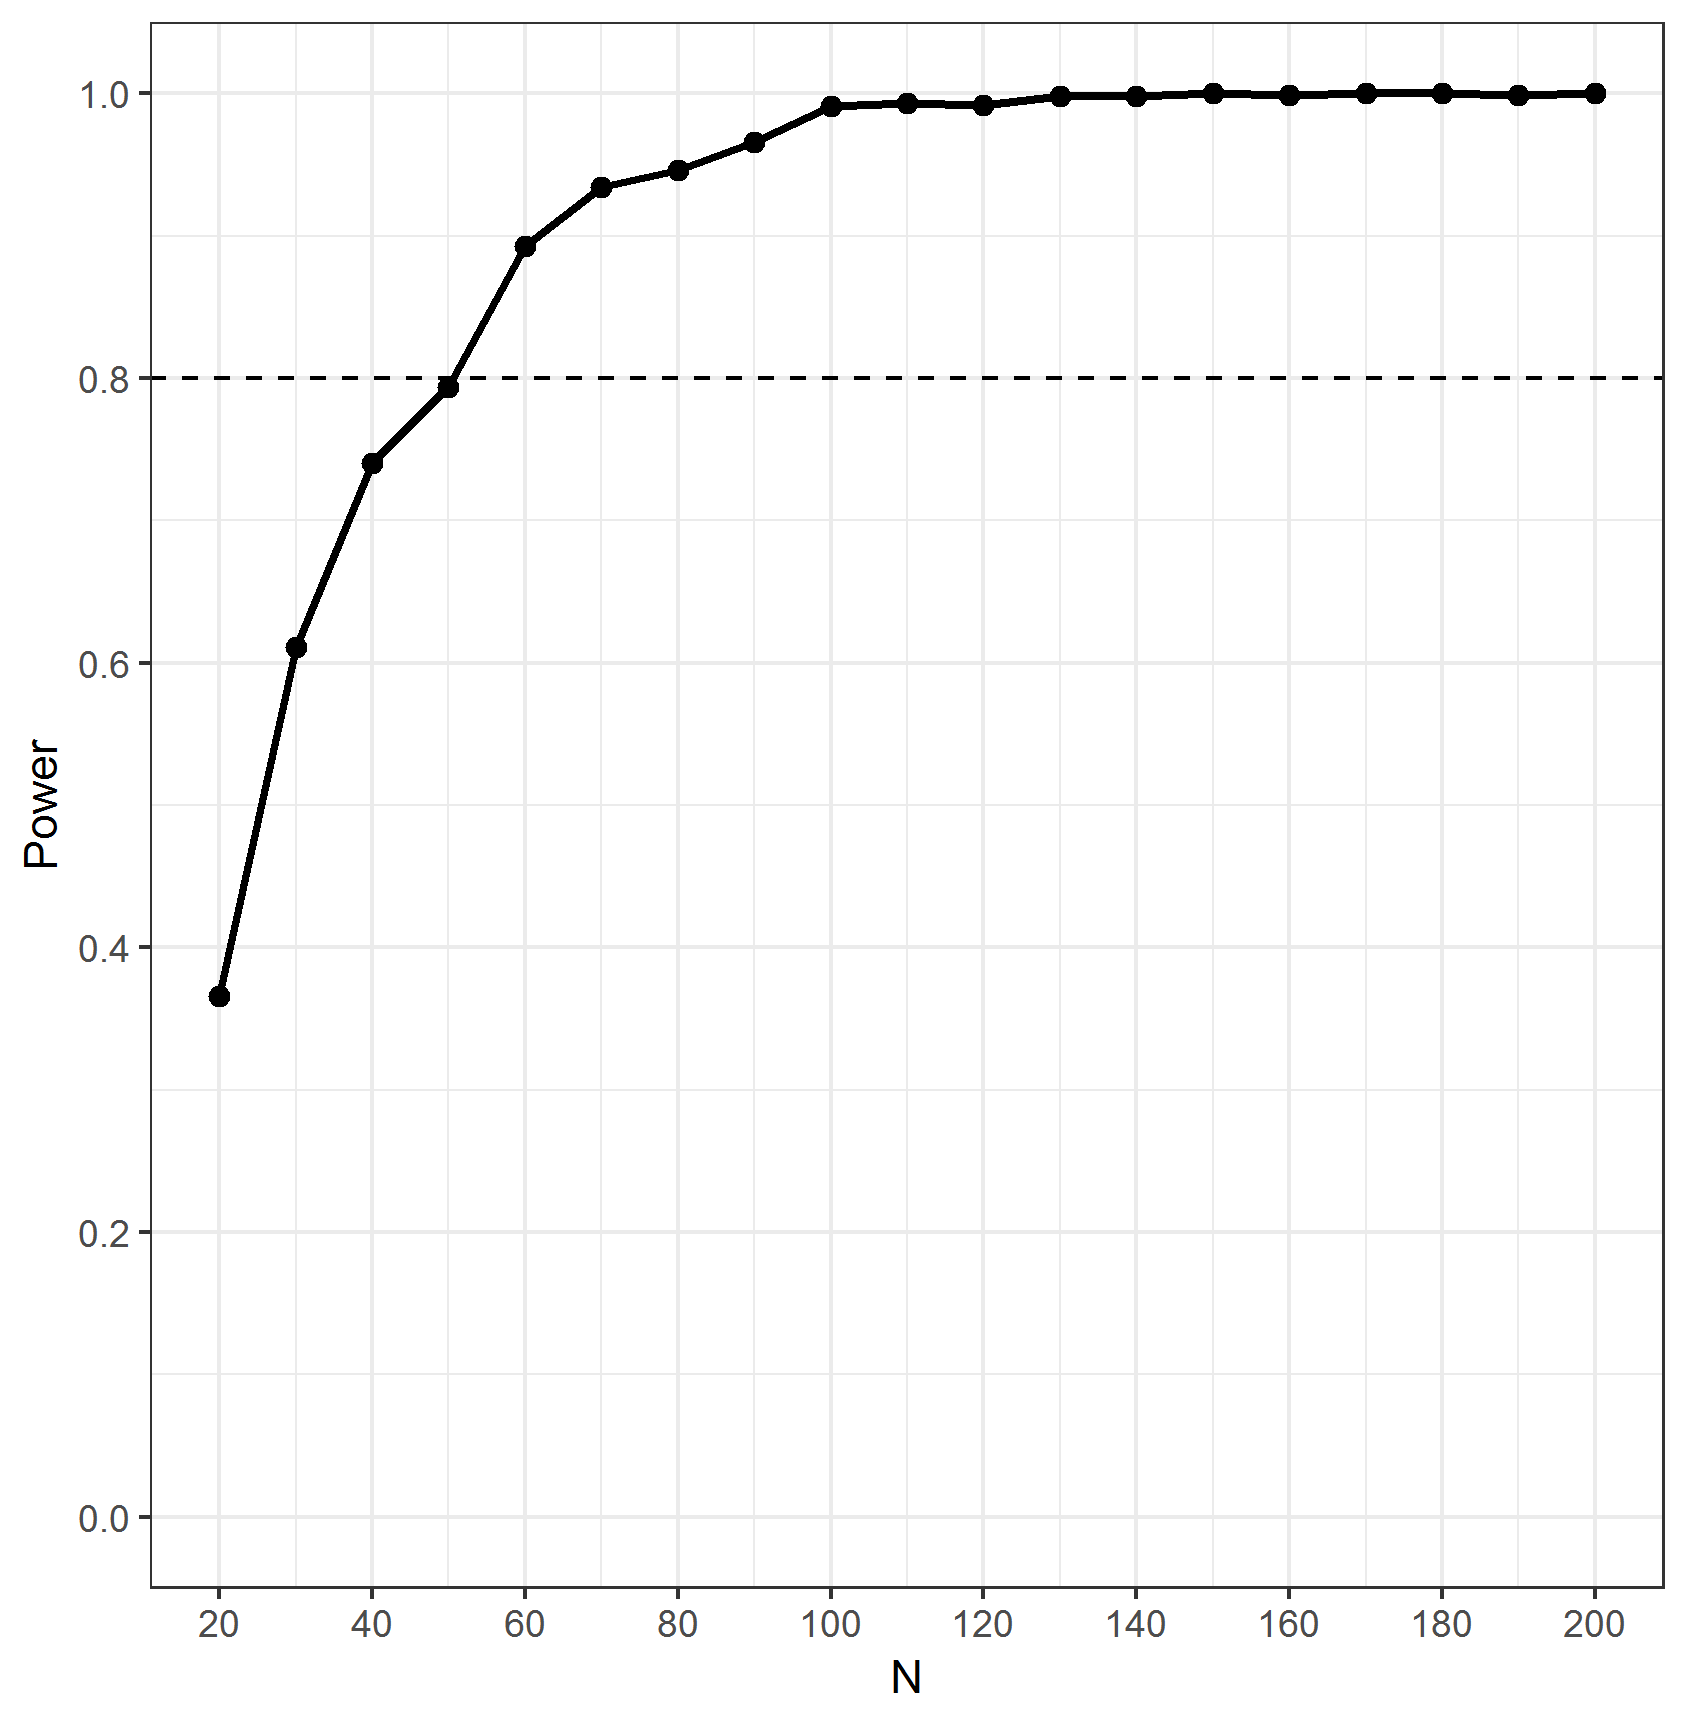
\includegraphics[width = \textwidth]{fig_power.png}
\caption{Power in dependence of sample size N. Power was estimated in a model--based power simulation where the true probability of using the Minkowski metric changed from 70\% to 30\% and the true probability of using the discrete metric changed from 30\% to 70\% when time pressure was introduced. To achieve the aspired power of .8, 60 participants (n=30 in each condition) were needed.}
\label{fig:power}
\end{figure}

\subsection{Procedure}
After arriving at the computer laboratory of the Center of Economic Psychology, participants were greeted, seated in front of a computer which was delimited from the other computers by dividing walls, and were provided with an informed consent which they could read through and sign in case of agreement. Upon signature, the experimenter typed in the participant id to start the experiment and the participant was presented a series of instructions on the computer (for the exact instructions, see \textit{appendix, still need to do this}. Participants first read, that they had to learn to assign different products to two different brands (brand L and brand R), that each product consisted of the same three ingredients but differed from other products in the specific ingredient quantities. They then saw a randomly chosen product (see Figure \ref{fig:material} for an example), read that each grey beam represented one ingredient and the number of colored squares in the beams indicated the quantity of the respective ingredient. To familiarize with the products, participants had to click on each ingredient at least ten times. With each click the quantity of the respective ingredient increased or decreased by one unit, ensuring that all participants saw all possible values on each feature. Participants then read that in each trial they would be presented with a random chosen product and their task was to correctly guess the brand of the respective product by pressing the left and right arrow keys. Participants read that the experiment consisted of two phases: In the first phase, they would learn the correct brand of each product and receive feedback after entering their answer. After achieving to consistently assign the products to the correct brand, they would reach the second phase and have to assign again several products to the brand to which they belonged most likely without receiving feedback. Participants in the time pressure condition furthermore read that they would have a time limit for their response in the second phase which they shouldn't exceed.

\subsubsection{Learning phase}
In the learning phase participants learned the category structure of eight products. All blocks of the learning phase included each of the eight products; the sequence within each block was randomized. In every trial participants could look at the given product for as long as they wished. Participants could then assign the product to brand L or R by pressing the left and right arrow key, respectively. Depending on the correctness of their response, participants received feedback in form of a happy, green smiley and the exclamation ''Richtig!'' (English: ''Correct!'') or in form of a sad, red smiley and the exclamation ''Falsch!'' (English: ''False!'') if their response was incorrect. Participants could continue looking at the product and the feedback for as long as they wished and then proceed to the next trial by pressing the upper arrow key. In case an invalid key was pressed, participants were reminded which keys to press to assign the product to a brand and to continue to the next trial. Figure \ref{fig:timeline} illustrates two trials of the learning phase.

After the first 100 learning trials participants received every 50 trials feedback on their accuracy in the last 100 trials. Participants needed to achieve the accuracy criterion which consisted of correctly classifying each stimulus the last three occurrences and 80\% accuracy in the last 100 trials. If participants didn't meet the accuracy criterion within an hour, the experiment was discontinued and the participants received appropriate course credit. Else, participants continued with the second phase.

\begin{figure}[htbp]
\centering
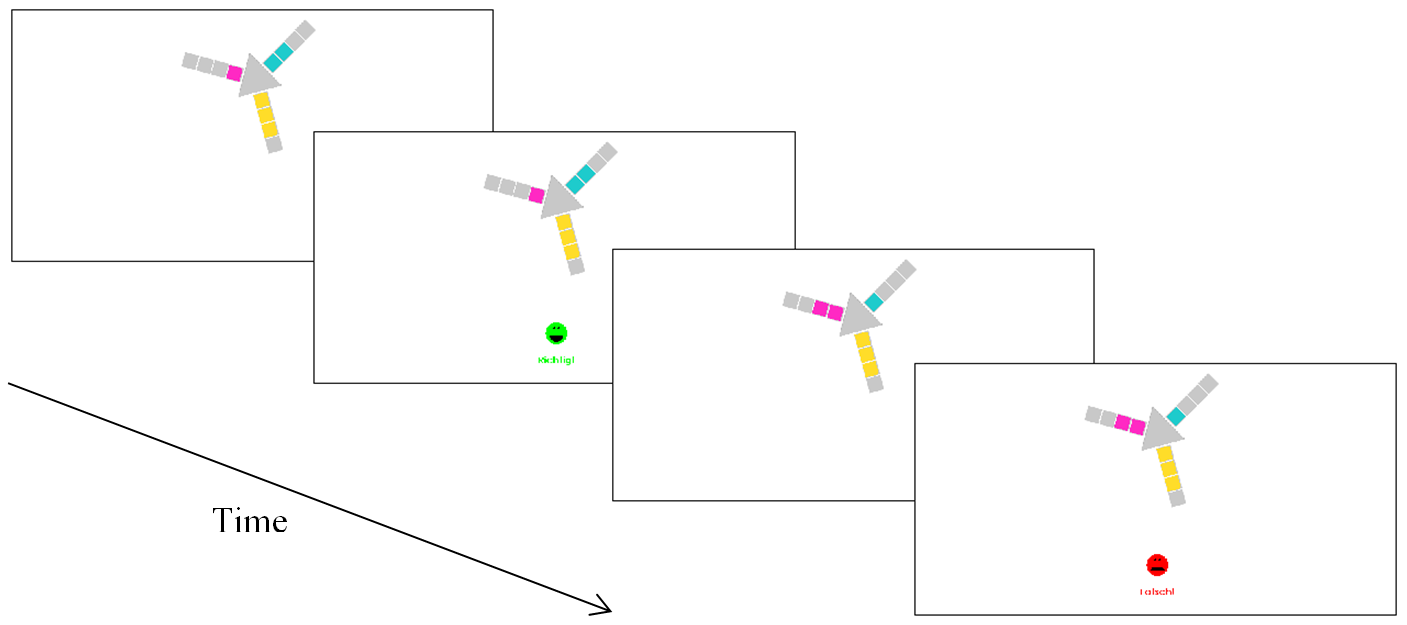
\includegraphics[width = \textwidth]{fig_timeline.png}
\caption{Timeline of the learning phase. Participants could look at at a given product for as long as they wished (first and third image) and enter their response via the left and right arrow keys. In case of a correct response, a happy, green smiley as well as ''Richtig!'' (English: ''Correct!'') appeared (second image). In case of an incorrect response, a sad, red smiley as well as ''Falsch!'' (English: ''False!'') appeared (forth image). In both cases, people could continue to look at the feedback for as long as they wished before proceeding to the next trial via the upper arrow key.}
\label{fig:timeline}
\end{figure}

\subsubsection{Test phase}
Participants were reminded that the second phase didn't include feedback anymore and in case of time pressure were provided with the lower and upper integer of the exact time they had per trial. Without time pressure, participants faced no response deadlines. Participants were informed that they will first perform some practice trials with already familiar products. Four blocks with the learning phase products in a randomized sequence per block were presented resulting in 32 familiarization trials. Upon completion, participants read that they should now assign further products to the two brands. Fourteen blocks consisting each of six novel and four familiar stimuli were presented resulting in 140 test trials. The sequence within each block was again randomized. The procedure in the test phase was equal to the one in the learning phase except that no feedback was provided, the following trial started 500 milliseconds after response entry, and a random half of participants had time pressure. If participants in the time pressure condition exceeded the time limit in a given trial they were informed that they were too slow and had to continue with the next trial after a 500 milliseconds inter--trial interval. After the test phase, participants filled out a questionnaire assessing key demographic variables (i.e., age, gender, education, and profession), vision (i.e., color blindness, impaired and corrected vision), and task--related characteristics (i.e., clearness of task and strategy used in the second phase). Participant then received appropriate course credit which marked the end of the experimental session.

\section{Results}
Figure \ref{fig:pred_obs_agg} illustrates for the six novel stimuli in the test phase the responses of participants separately for each time pressure condition as well as the predictions of the generalized context model with both the Minkowski and the discrete metric as well as the multidimensional and the unidimensional version across all parameter combinations reaching the accuracy criterion.

\begin{figure}[htbp]
\centering
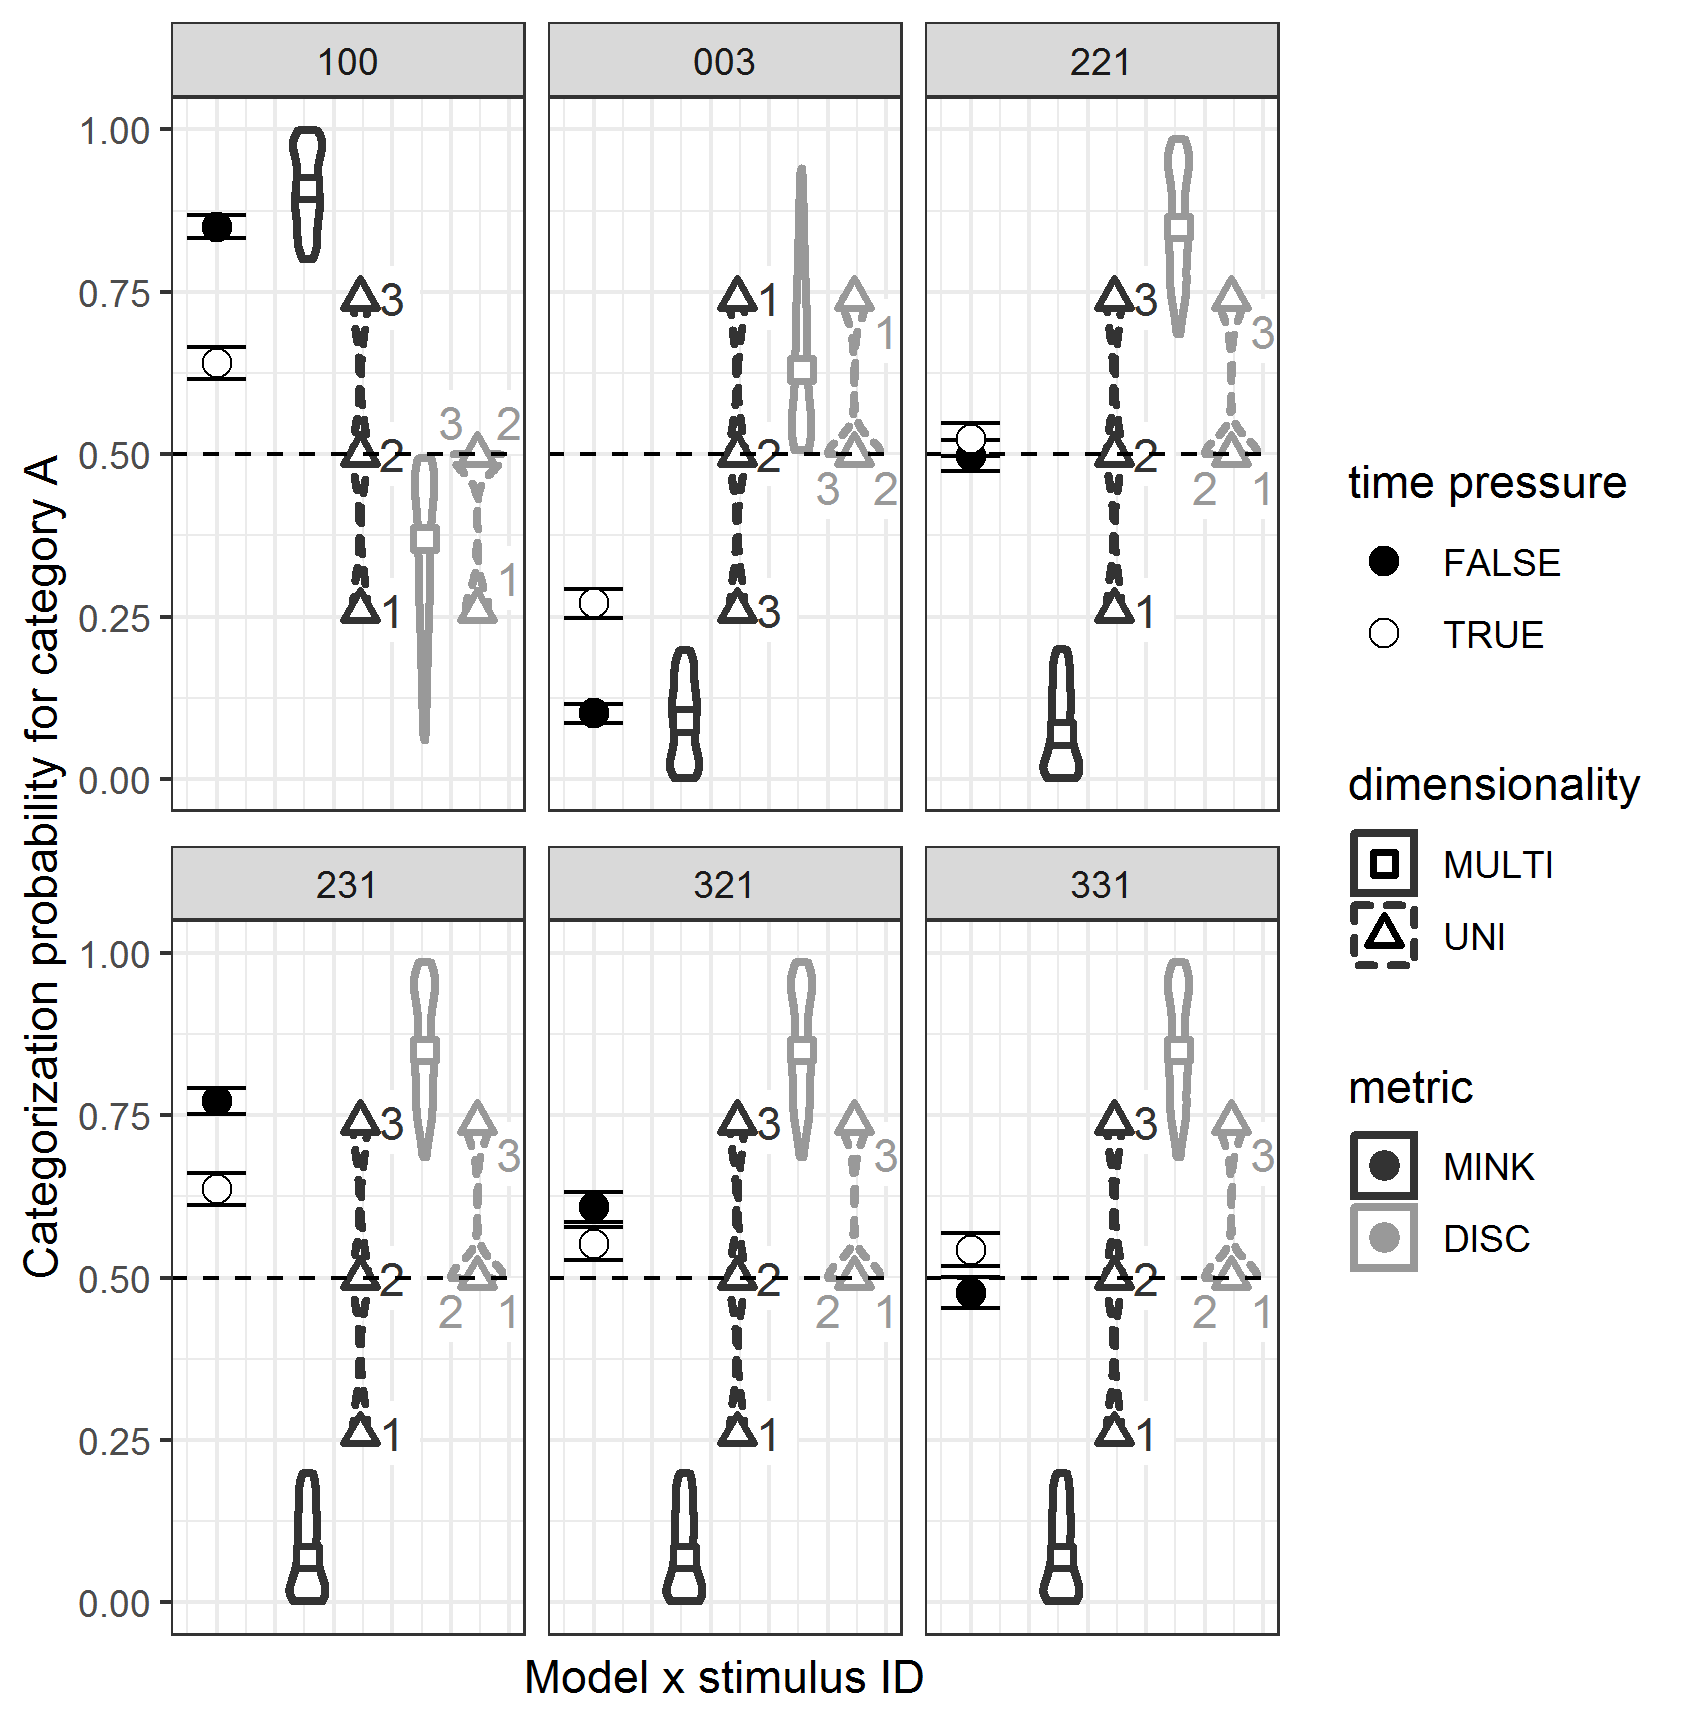
\includegraphics[width = \textwidth]{fig_pred_obs_agg.png}
\caption{Predicted and observed responses for the novel stimuli of the test phase. Points and errorbars on the left denote the mean response and the standard error across participants for each stimulus separately for each time pressure condition. The four violins on the right denote model predictions for all parameter combinations reaching the accuracy criterion. The shapes within the violins denote the median model predictions.}
\label{fig:pred_obs_agg}
\end{figure}

For all statistical tests, an alpha level of .05 was used, except when multiple comparison corrections are indicated. Analyses included inferential tests at the aggregate level and cognitive modeling at the aggregate and individual levels.

\subsection{Inferential tests at the aggregate level}
A linear mixed model with logit link was fitted to the observed responses to the novel stimuli in the test phase using the lme4 R package. As the model did not converge in its preregistered form, I diminished the number of estimated parameters. Specifically, we took together the stimuli 221, 231, 321, and 331 for whom the model predictions were similar and fitted a random intercept, but no random slope per participant instead of the preregistered random slope, but no random intercept. The final model included the fixed effects time pressure condition, stimulus (with three levels), and the interaction thereof and has participant as random effect. The interaction between time pressure and stimulus, postulated by H1 and H2, was tested with relative AIC weights \citep[][p. 194]{wagenmakers2004aic} and was found necessary as the full model with the interaction term had $5.36 * 10^{36}$ higher AIC weights than a restricted model without the interaction term. A supplementary model comparison using ANOVA yielded as well the superiority of the model with the interaction term ($\chi^{2}(2)$ = 145.51, $p$ < .001). 

The following tests refer to the coefficients of the full model with category A being coded as 1. We preregistered to accept H1a, H1b, H1c, and H2a, respectively, in case of a change of algebraic sign or a significant one-sided contrast when comparing a particular stimulus of interest with the remaining novel stimuli of the test phase. The alpha level for the statistical tests of the contrasts was corrected using the Holm--Bonferroni method \citep{holm1979simple}. H1a (people use the discrete metric under time pressure) predicted that the coefficient of stimulus 100 was the only negative coefficient or significantly lower than the remaining coefficients given time pressure. H1b (people use a unidimensional Minkowski metric under time pressure) predicted that the coefficient of stimulus 003 differed from the remaining stimuli in one of the aforementioned ways, irrespective of the coefficients' direction. H1c predicted reverse directions of the coefficients' signs compared to H1a. Analyses of the logit least--square means for the time pressure condition (0.73 for stimulus 100, -1.24 for stimulus 003, and 0.30 for the four combined stimuli) yielded the following results: H1a was rejected as the coefficient of stimulus 100 was positive and significantly higher than the remaining coefficients ($p$ < .001). H1b was accepted as the coefficient of stimulus 003 was significantly lower than the remaining coefficients ($p$ < .001). H1c was accepted due to the significant contrast between stimulus 100 and the remaining stimuli. These results thus support the use of a Minkowski metric on the aggregate level given time pressure, with the unidimensional version fulfilling both acceptance criteria and the multidimensional version fulfilling a significant contrast. H2a (people use the multidimensional Minkowski metric without time pressure) predicted that the coefficient of stimulus 100 was the only positive coefficient or significantly higher than the remaining coefficients given no time pressure. Analyses of the logit least--square means for the no time pressure condition (2.52 for stimulus 100, -3.02 for stimulus 003, and 0.52 for the four combined stimuli) yielded: H2a was accepted as the coefficient of stimulus 100 was significantly higher than the remaining coefficients ($p$ < .001). These results thus support the use of a multidimensional Minkowski metric on the aggregate level given no time pressure.

\subsection{Cognitive modeling}
To test the remaining hypotheses, cognitive modeling was employed. During the modeling all fitting used maximum likelihood. Model parameters were as follows: The generalized context model with the multidimensional Minkowski metric and the multidimensional discrete metric had both five parameters (three attention weights $w$s, the sensitivity parameter $c$, and the softmax choice-rule parameter temperature $\tau$). The unidimensional model with Minkowski metric and the discrete metric had both three parameters (which attention weight $w$ is set to 1, $c$, and $\tau$ defined as before). The decay parameter $p$ and the exponent of the distance metric $r$ were fixed to 1 for all model versions, as the experiment used discriminable stimuli with separable features. 

The parameters of the generalized context model with the multidimensional Minkowski metric and the multidimensional discrete metric were fit to individual participants’ learning phase data. After fitting, the parameters of both model versions were fixed to the resulting optimal parameters for each participant. The attention weight parameter of the unidimensional models was fit to individual participants’ test phase data. To avoid over--fitting, the sensitivity parameter $c$ and temperature $\tau$ of the unidimensional models were not fitted, but fixed to the corresponding multidimensional model’s parameter estimates for each participant. The distribution of fitted parameters across participants is shown in Figure \ref{fig:par_multidim} for the multidimensional model and in Figure \ref{fig:par_unidim} for the unidimensional model versions. 

\begin{figure}[htbp]
\centering
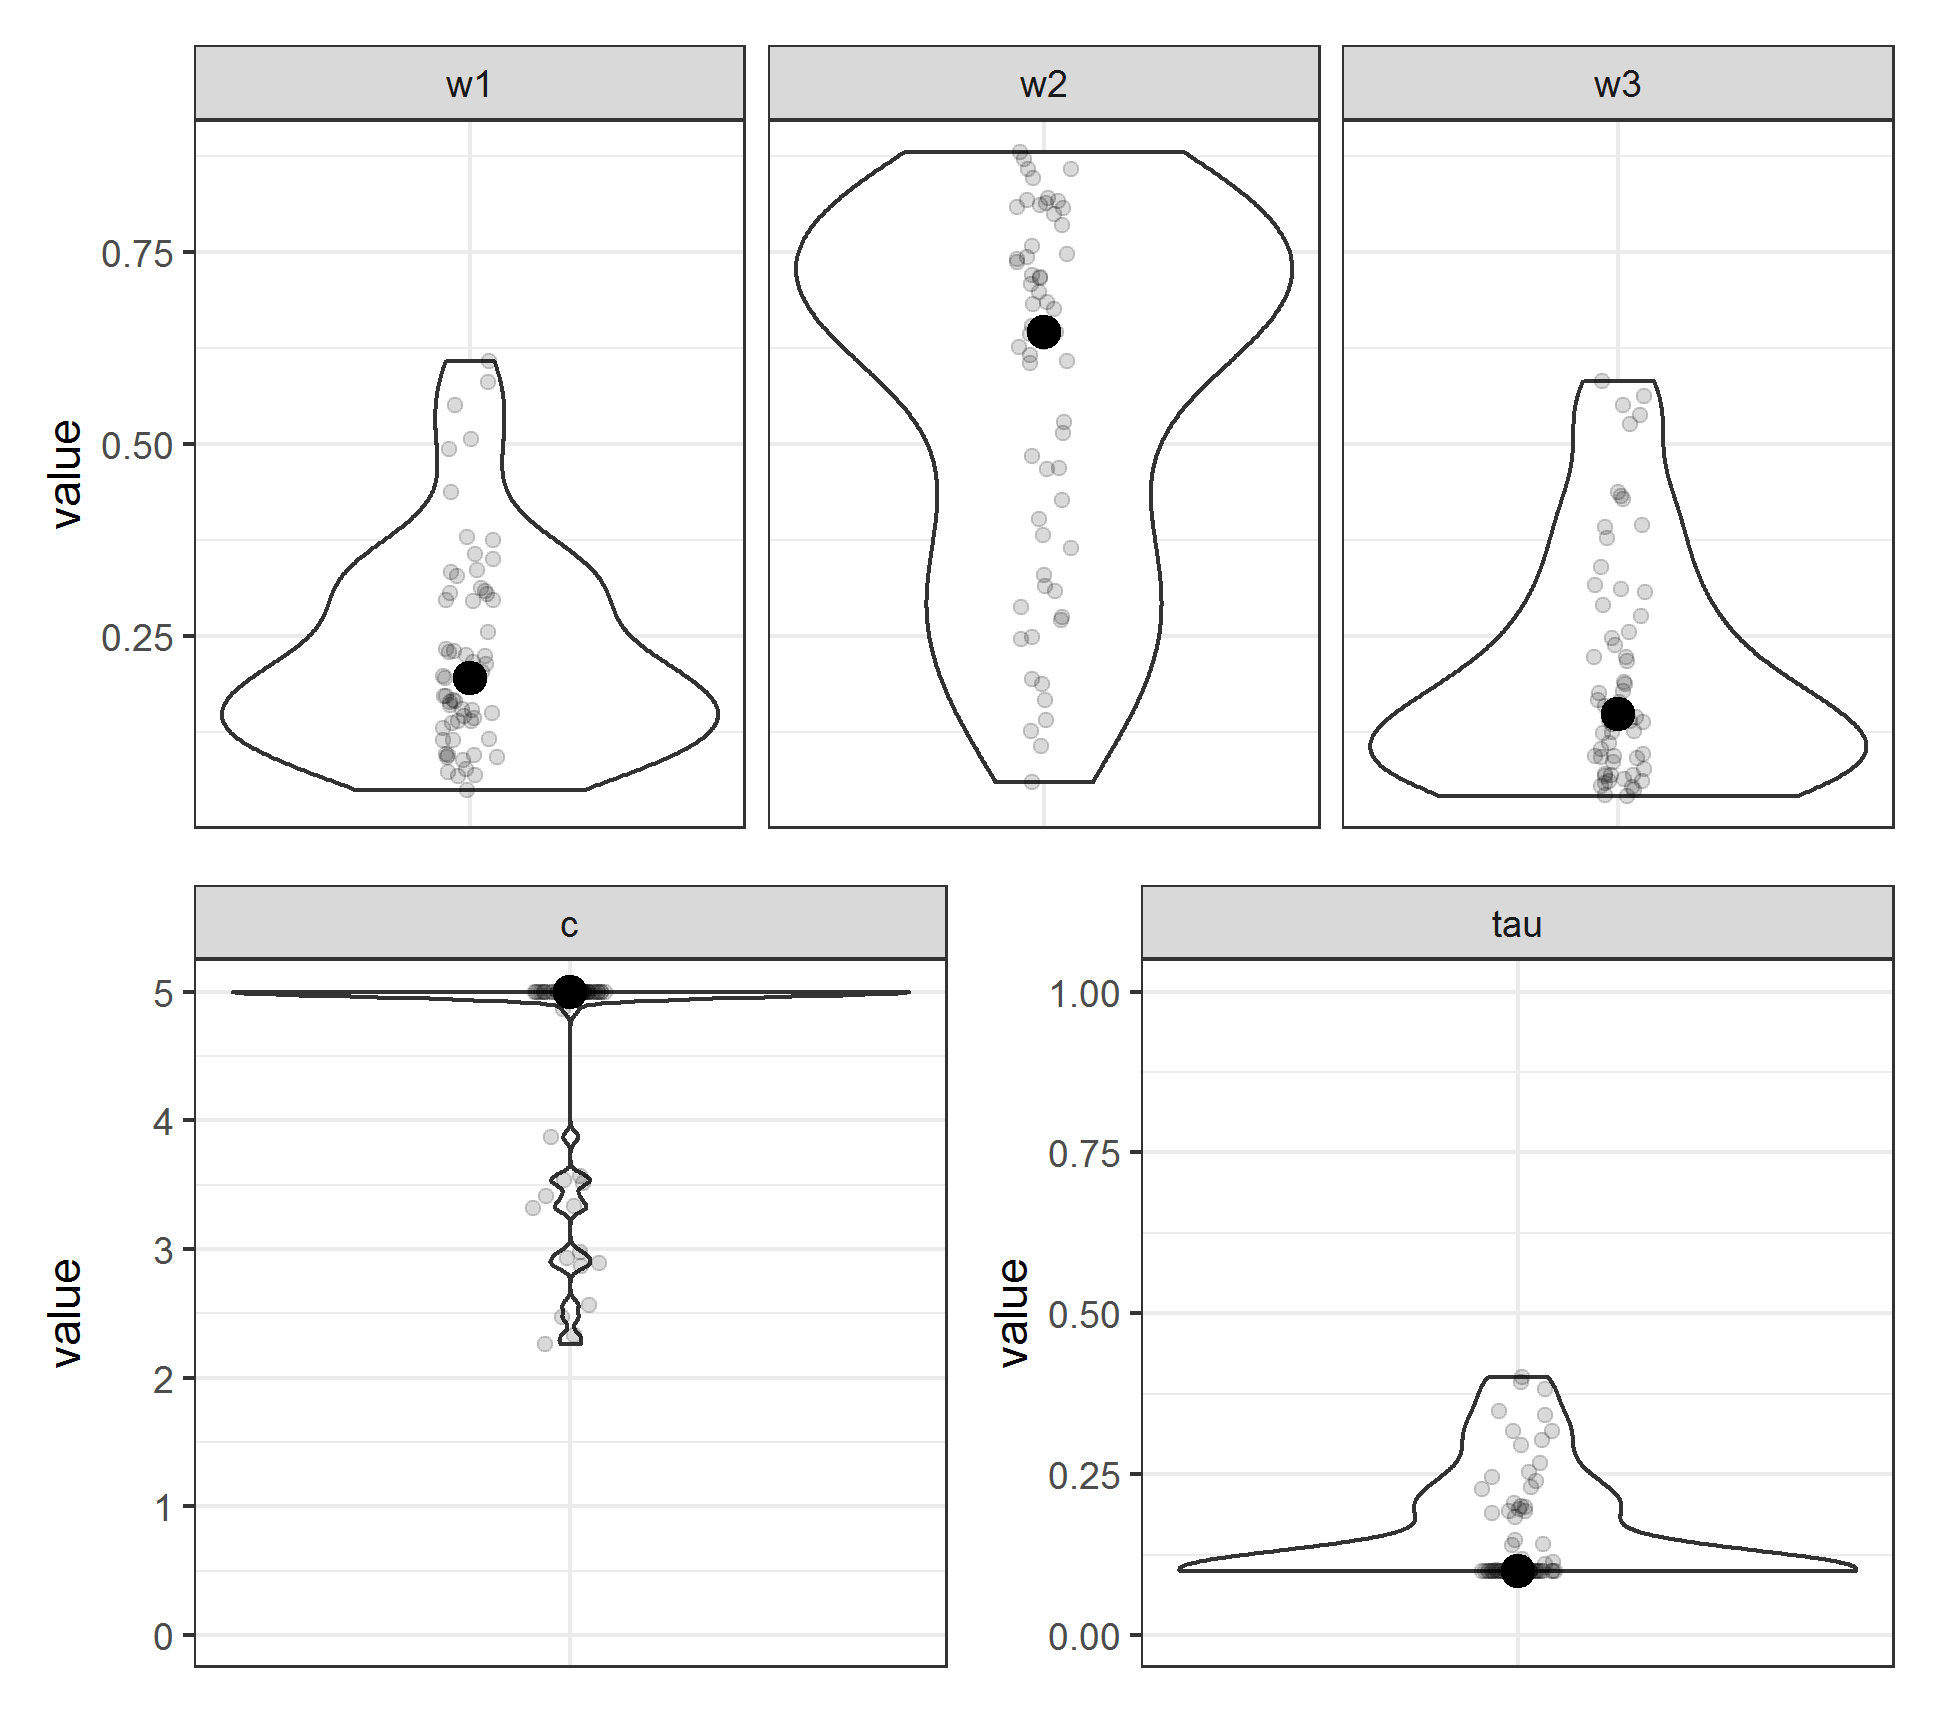
\includegraphics[width = \textwidth]{fig_par_multidim.png}
\caption{Distribution of parameter estimates for the multidimensional generalized context model. Grey shaded points within the violins indicate individual parameter estimates, the large point within each violin indicates the median parameter estimate across participants.}
\label{fig:par_multidim}
\end{figure}

\begin{figure}[htbp]
\centering
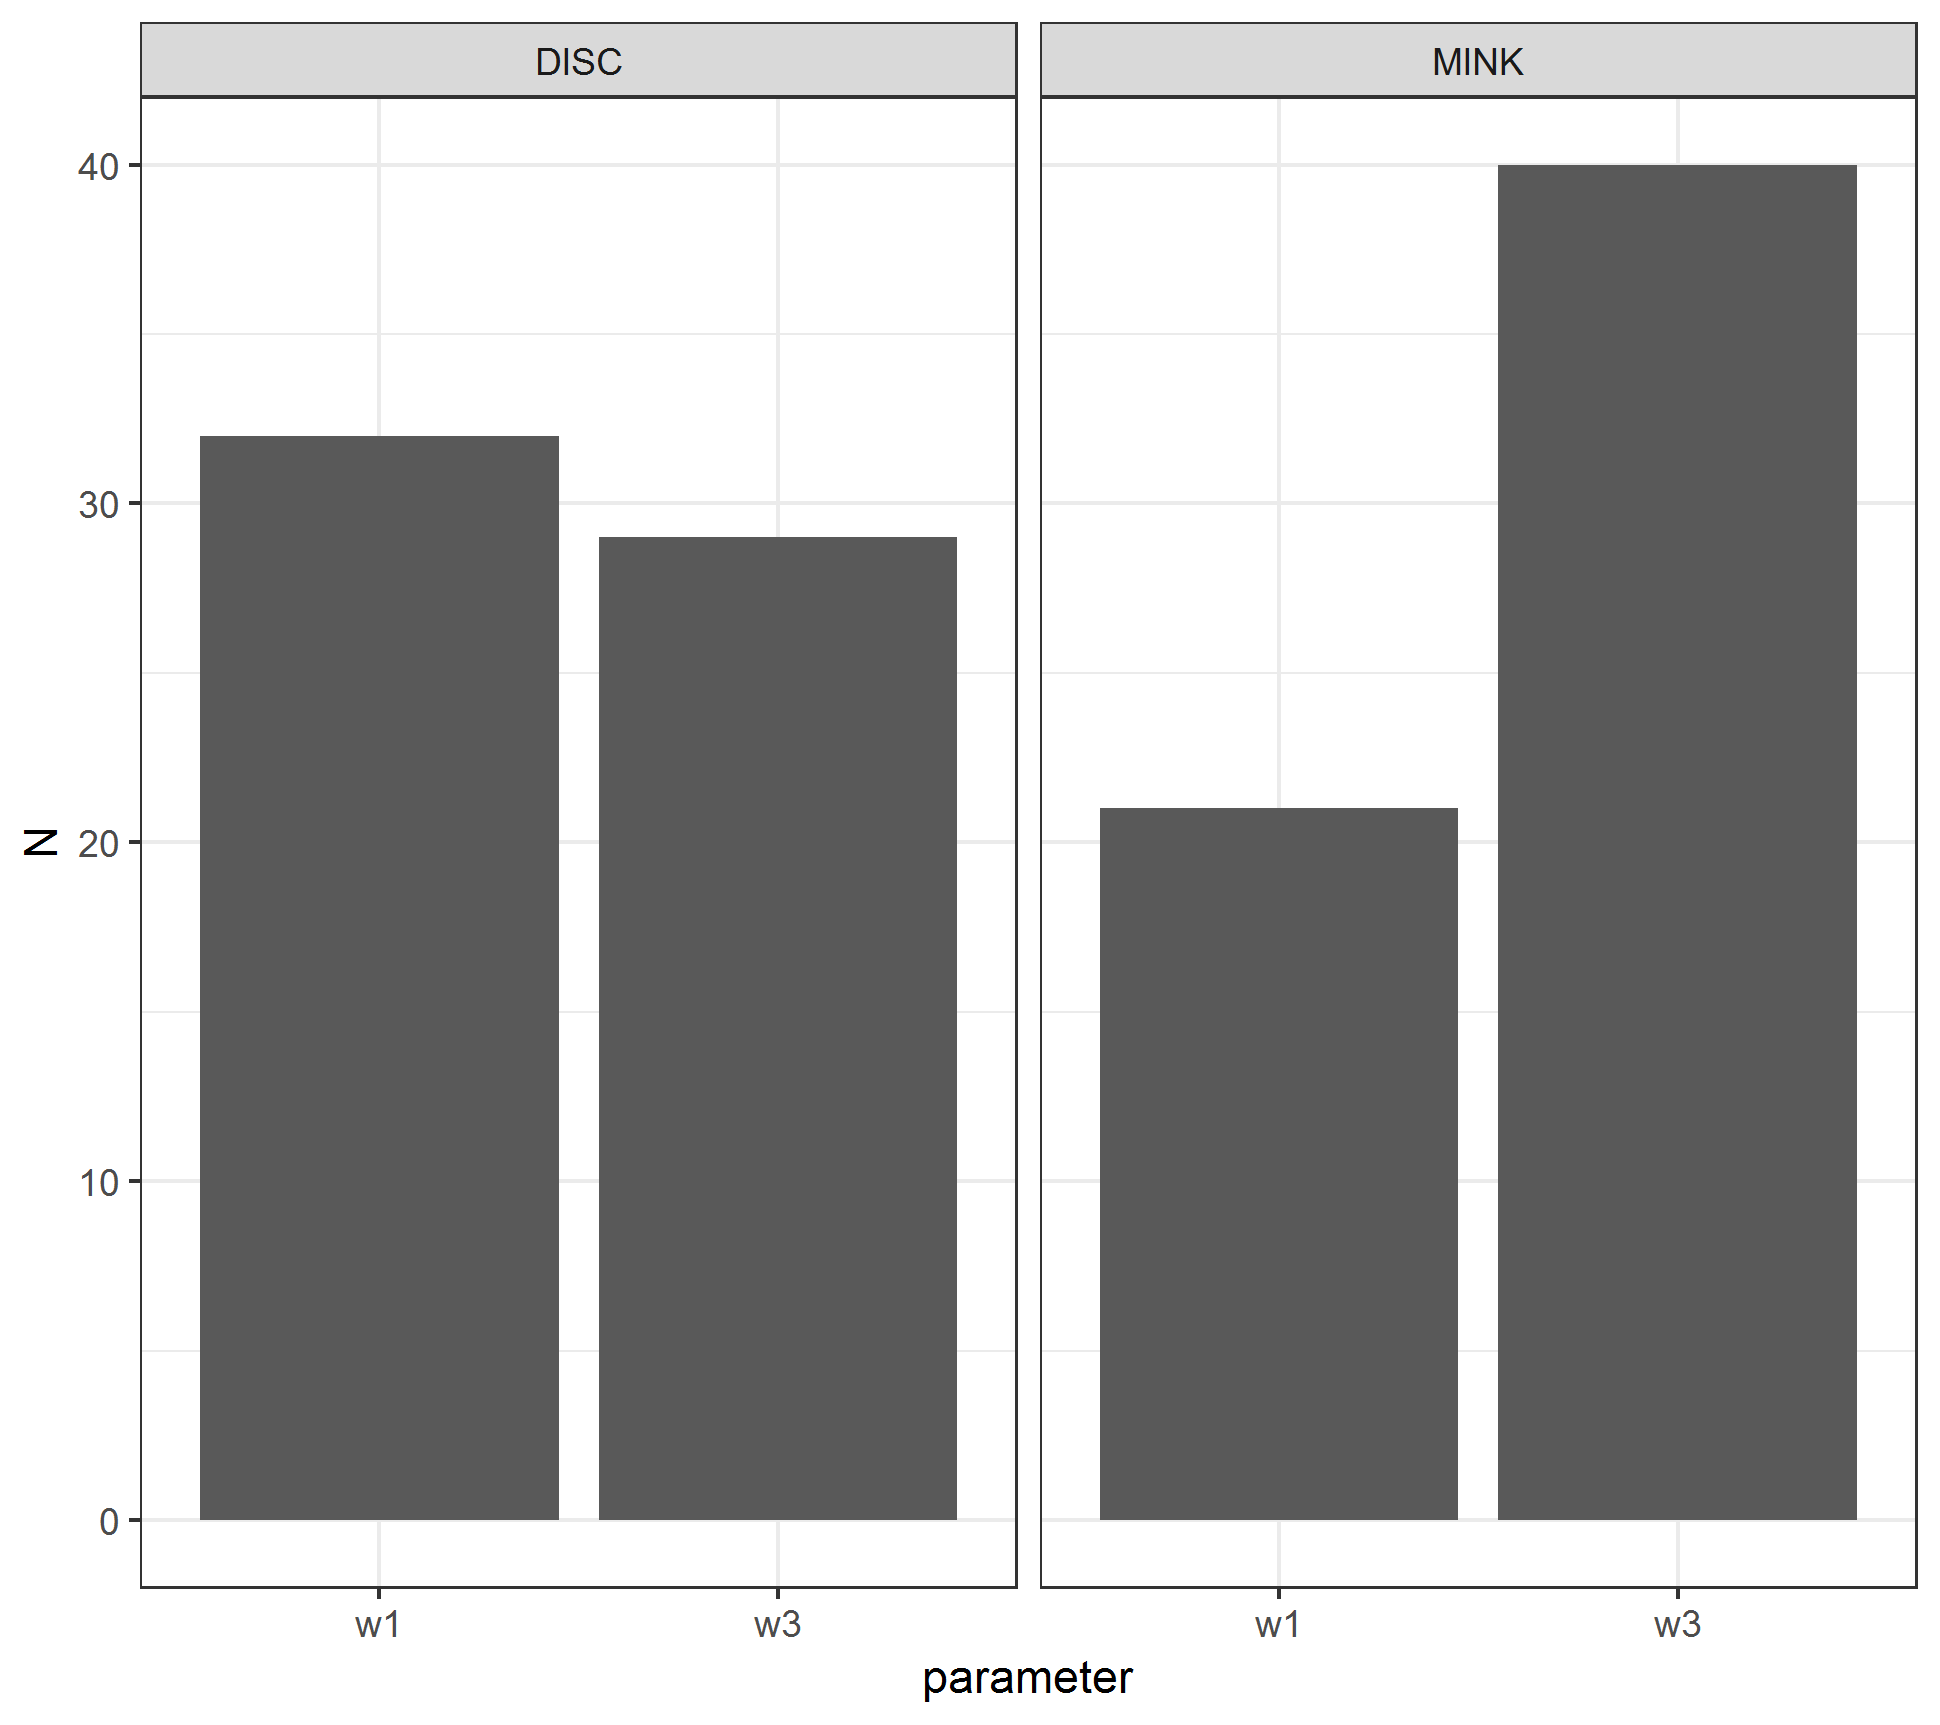
\includegraphics[width = \textwidth]{fig_par_unidim.png}
\caption{Distribution of attention weight estimates for the unidimensional generalized context model. Bars indicate separately for the Minkowski metric and the discrete metric how many people are best described by full attention to the first and the third feature, respectively. Full attention to the second feature wasn't included as this model couldn't be discriminated from a random choice model. Parameter estimates of $c$ and $\tau$ were taken from the participants' respective optimal parameter estimates in the multidimensional generalized context model.}
\label{fig:par_unidim}
\end{figure}

Participants centered much attention on the second dimension, had very high sensitivity and very low temperature at the boundary of the valid range of the respective parameters which points towards many corner point solutions. For the unidimensional discrete model, 32 participants were best fit by the model with full attention on the first dimension, 29 by the model with full attention on the third dimension ($\chi^{2}(1)$ = 0.15, $p$ = .70). For the unidimensional Minkowski model, 21 participants were best fit by the model with full attention on the first dimension, 40 by the model with full attention on the third dimension ($\chi^{2}(1)$ = 5.92, $p$ = .01).

The following model comparison included the multidimensional model with the discrete metric and the Minkowski metric, the unidimensional model with the discrete metric and the Minkowski metric, and a baseline random choice model. If a unidimensional strategy attending to the second dimension described a participant best, we assumed they followed a random choice model, because in our design these two models couldn't be distinguished. 

\subsubsection{Model comparison at the aggregate level} \label{sec:res_agg}
For each model, using each participant's optimal parameters, the median log likelihood of the observed test phase data was computed from the models' predictions separately for the condition with and without time pressure. The median log likelihoods were transformed into evidence strengths \citep[Akake weights,][]{wagenmakers2004aic}, and pairwise comparisons between models were conducted \citep[as in][p. 194]{wagenmakers2004aic}. To determine the rank order of models, a model was accepted as superior to another model if its evidence ratio (normalized probability of one model over the other) in the paired comparison exceeded .90, rejected if it was inferior to .10; otherwise inconclusive evidence resulted. 

Using the data with time pressure, the rank order hypothesized in H1d (the multidimensional and unidimensional discrete metric on the first rank, the unidimensional Minkowski metric on the second rank, the multidimensional Minkowski metric on the third rank, and the random choice model on the final rank) couldn't be established. Specifically, the random model outperformed the remaining models, followed by the multidimensional discrete model on the second rank, the multidimensional Minkowski model on the third rank, and the unidimensional discrete model as well as the unidimensional Minkowski model on the final rank. 

Also without time pressure, the rank order hypothesized in H2b (the multidimensional Minkowski metric on the first rank and the random choice model on the last rank) couldn't be demonstrated. Specifically, the multidimensional discrete model exceeded the remaining models, followed by the multidimensional Minkowski model on the second rank, the random choice model on the third rank, the unidimensional Minkowski model on the forth rank, and the unidimensional discrete model on the final rank. Both H1d and H2b were thus rejected.

Table 2 shows the median log likelihood as well as mean and the standard deviation of the log likelihood, the mean absolute prediction error ($MAPE$), the mean accuracy based on the arg max choice rule, and the mean--square error ($MSE$) for the different models separately for the conditions with and without time pressure. Figure \ref{fig:log_lik} further illustrates the negative log likelihoods of the test phase data for the different models separately for the conditions with and without time pressure.

\begin{sidewaystable}
\begin{center}
\begin{threeparttable}
\caption{Descriptive model fit measures}
\label{tab:fitmeasures}
\begin{tabular}{llcccccccccccc}
\toprule
 &  & \multicolumn{6}{c}{Time pressure} & \multicolumn{4}{c}{No time pressure}\\
\cmidrule(r){3-8} \cmidrule(r){9-14}
 &  & \multicolumn{3}{c}{Log likelihood} & & & & \multicolumn{3}{c}{Log likelihood} & & & \\
\cmidrule(r){3-5} \cmidrule(r){9-11}
Dimensionality & \multicolumn{1}{l}{Metric} & \multicolumn{1}{c}{$M$} & \multicolumn{1}{c}{$M$} & \multicolumn{1}{c}{$SD$} & \multicolumn{1}{c}{$MAPE$} & \multicolumn{1}{c}{$Arg max$} & \multicolumn{1}{c}{$MSE$} & \multicolumn{1}{c}{$M$} & \multicolumn{1}{c}{$Md$} & \multicolumn{1}{c}{$SD$} & \multicolumn{1}{c}{$MAPE$} & \multicolumn{1}{c}{$Arg max$} & \multicolumn{1}{c}{$MSE$}\\
\midrule
\addlinespace
\multicolumn{2}{l}{\emph{Generalized Context Model}} \\
\addlinespace
\multirow{2}{*}{Multidim} & Discrete & -115.53 & -110.25 & 28.52 & 0.47 & 0.51 & 0.31 & -84.58 & -79.60 & 29.85 & 0.38 & 0.63 & 0.21\\
\cmidrule(r){2-14}
 & Minkowski & -137.07 & -120.97 & 60.07 & 0.47 & 0.53 & 0.34 & -106.25 & -94.25 & 54.72 & 0.36 & 0.69 & 0.24\\
\cmidrule(r){1-14}
\multirow{2}{*}{Unidim} & Discrete & -160.29 & -150.89 & 66.27 & 0.42 & 0.51 & 0.32 & -181.95 & -151.16 & 83.10 & 0.46 & 0.52 & 0.34\\
\cmidrule(r){2-14}
 & Minkowski & -163.57 & -149.03 & 83.47 & 0.34 & 0.69 & 0.29 & -163.04 & -132.58 & 86.10 & 0.34 & 0.68 & 0.29\\
\cmidrule(r){1-14}
\multicolumn{2}{l}{\emph{Random Choice Model}} & -89.79 & -93.23 & 7.76 & 0.50 & 0.00 & 0.25 & -97.04 & -97.04 & 0.00 & 0.50 & 0.00 & 0.25\\
\bottomrule
\addlinespace
\end{tabular}
\begin{tablenotes}[para]
\textit{Note.} Different fit measures for the different models separately for the conditions with and without time pressure. 
          Fit measures are the following: $M$ = mean log likelihood, $Md$ = median log likelihood, $SD$ = standard deviation of log likelihood, $MAPE$ = mean absolute percentage error, $Arg max$ = mean accuracy based on the arg max choice rule, $MSE$ = mean--square error.
\end{tablenotes}
\end{threeparttable}
\end{center}
\end{sidewaystable}

\begin{figure}[htbp]
\centering
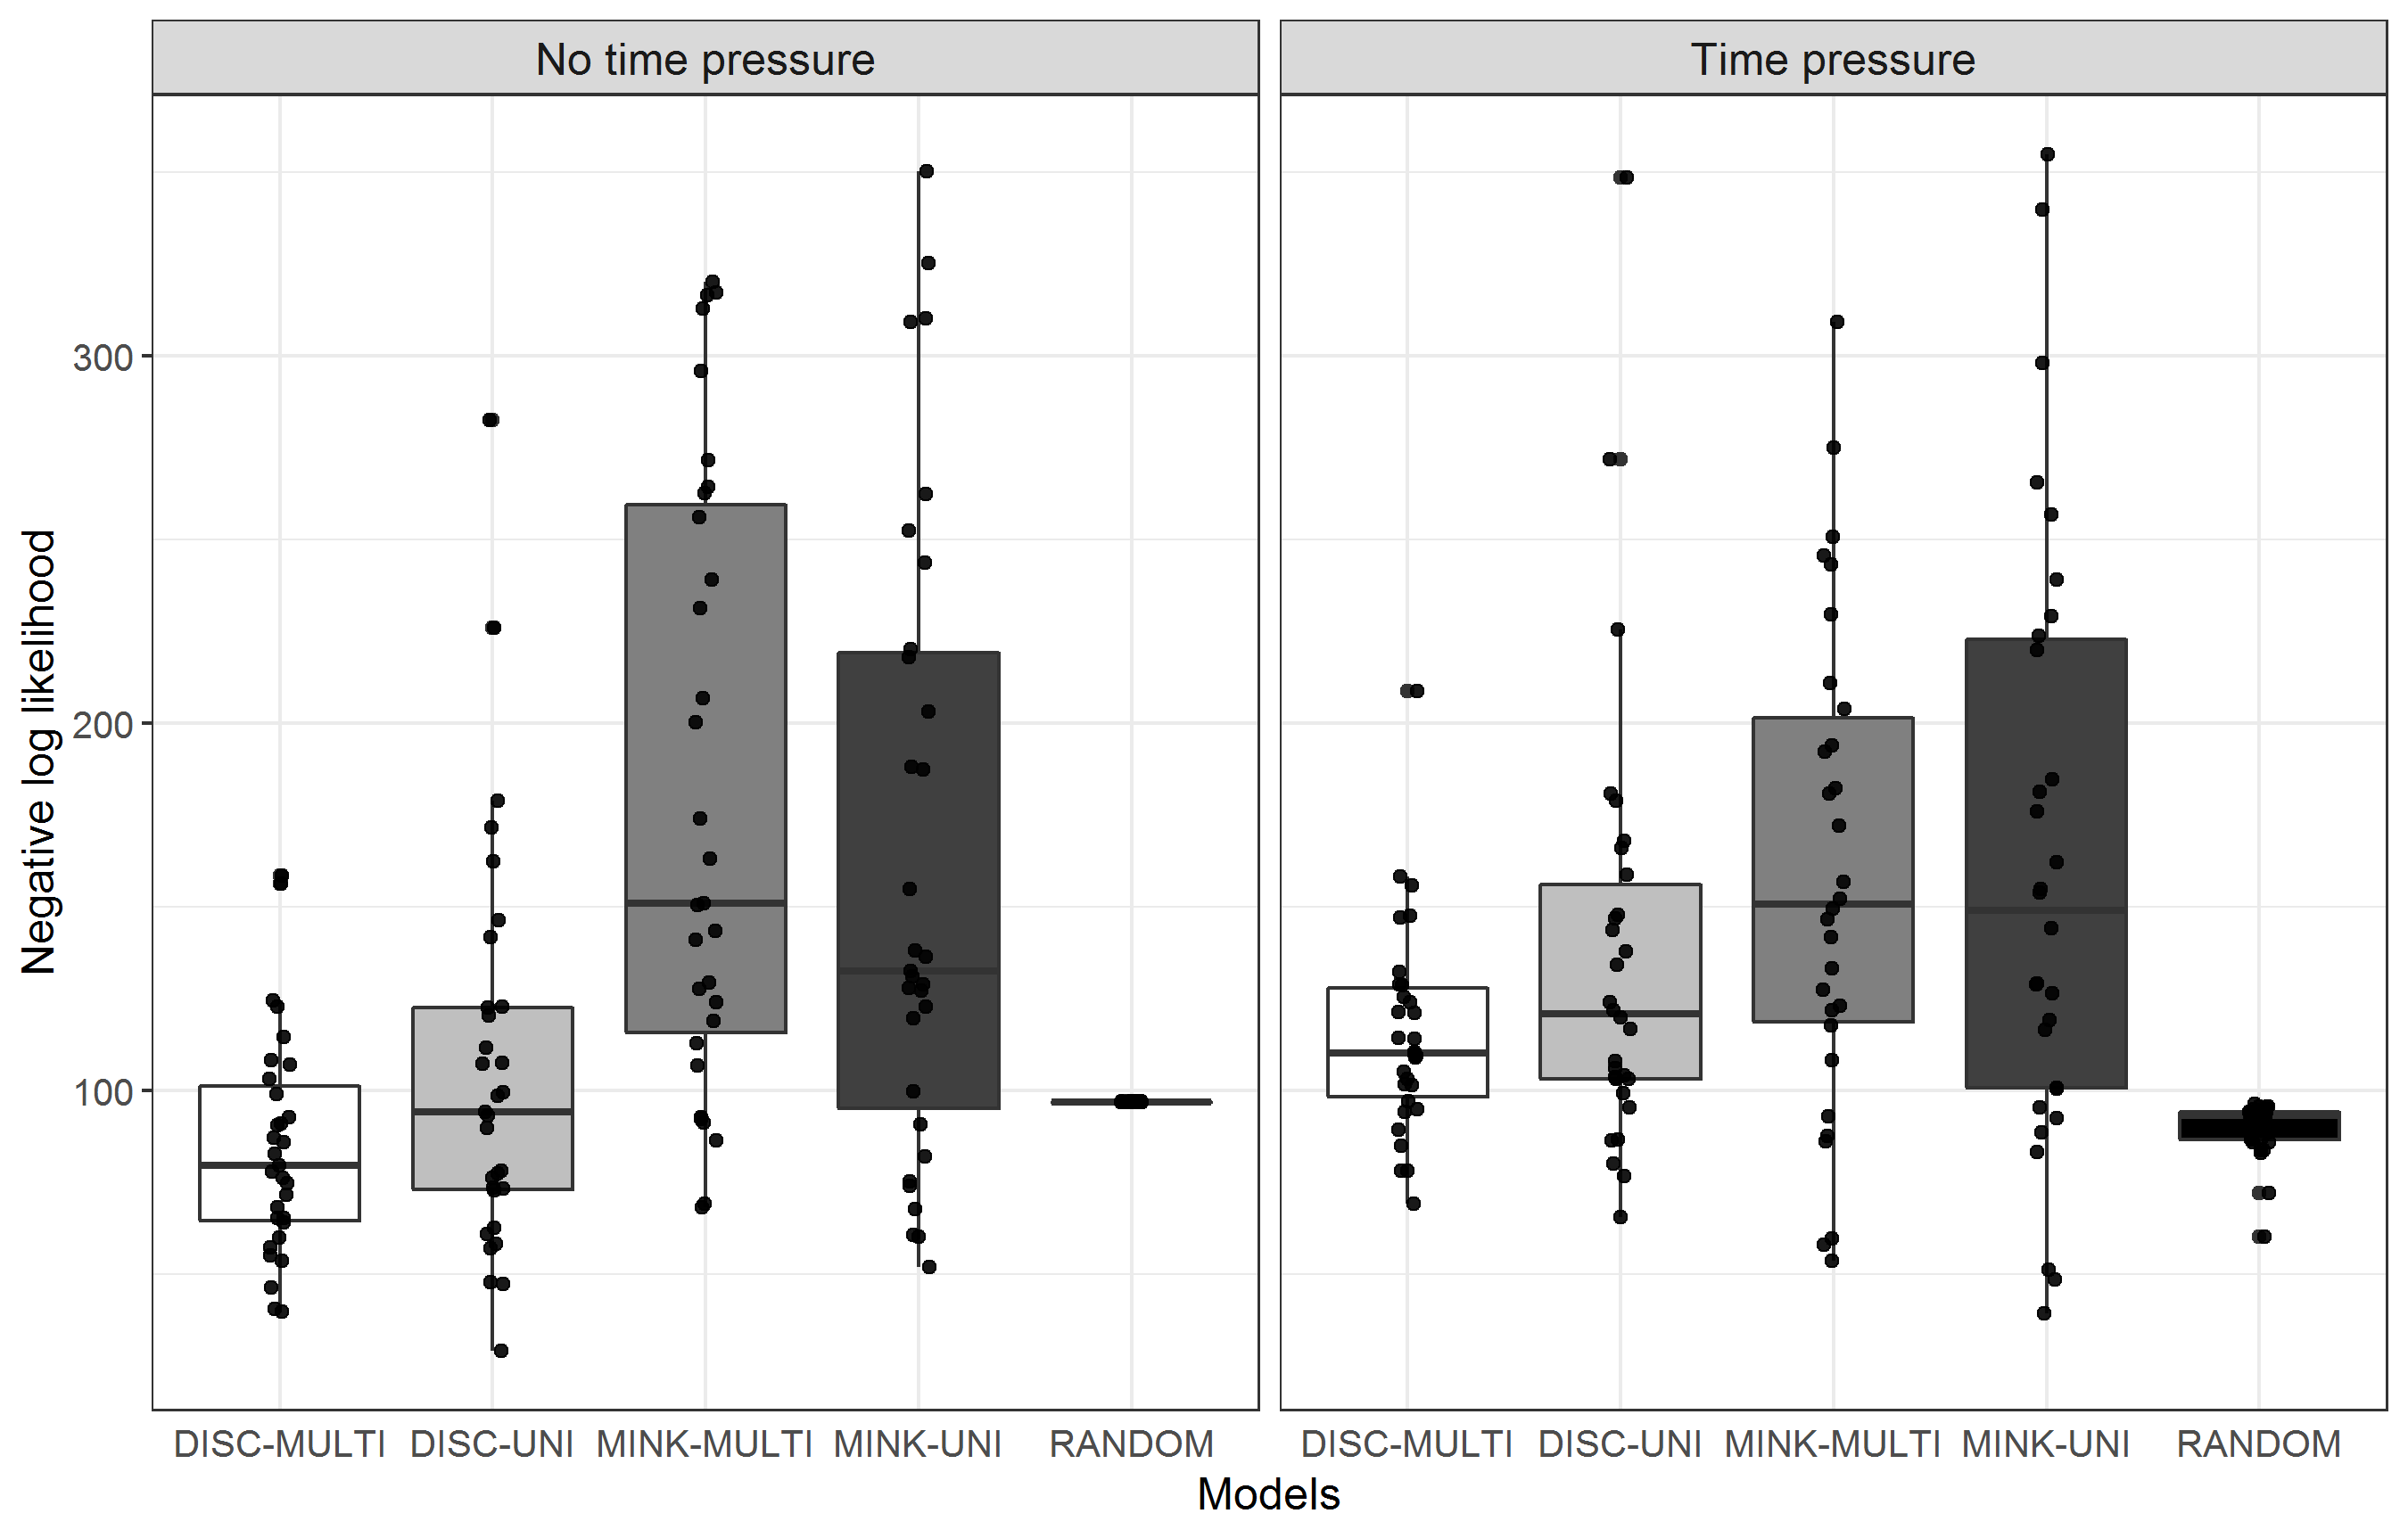
\includegraphics[width = \textwidth]{fig_log_lik.png}
\caption{Negative log likelihood of the test phase data given model predictions for both time pressure conditions. Lower values indicate a better fit of the model to the test phase data. Points illustrate the individual negative log likelihoods. DISC and MINK denote the discrete metric and the Minkowski metric, respectively. MULTI and UNI denote multidimensional and unidimensional model versions, respectively. RANDOM = random choice model.}
\label{fig:log_lik}
\end{figure}

\subsubsection{Model comparison at the individual level} \label{sec:res_ind}
For each model, using each participant's optimal parameters, the log likelihood of the test phase data was computed per participant. Individual log likelihoods were transformed into Akaike weights \citep{wagenmakers2004aic} and individual strategy classification was conducted on these Akaike weights. Specifically, if any model’s Akaike weight exceeded .90 the person was assigned to that model; else the person was classified as not described by any model. The resulting distribution of participants assigned to models is shown in Figure \ref{fig:model_selection}. Figure \ref{fig:aic} further shows for each participant the Akaike weights of the different models.

\begin{figure}[htbp]
\centering
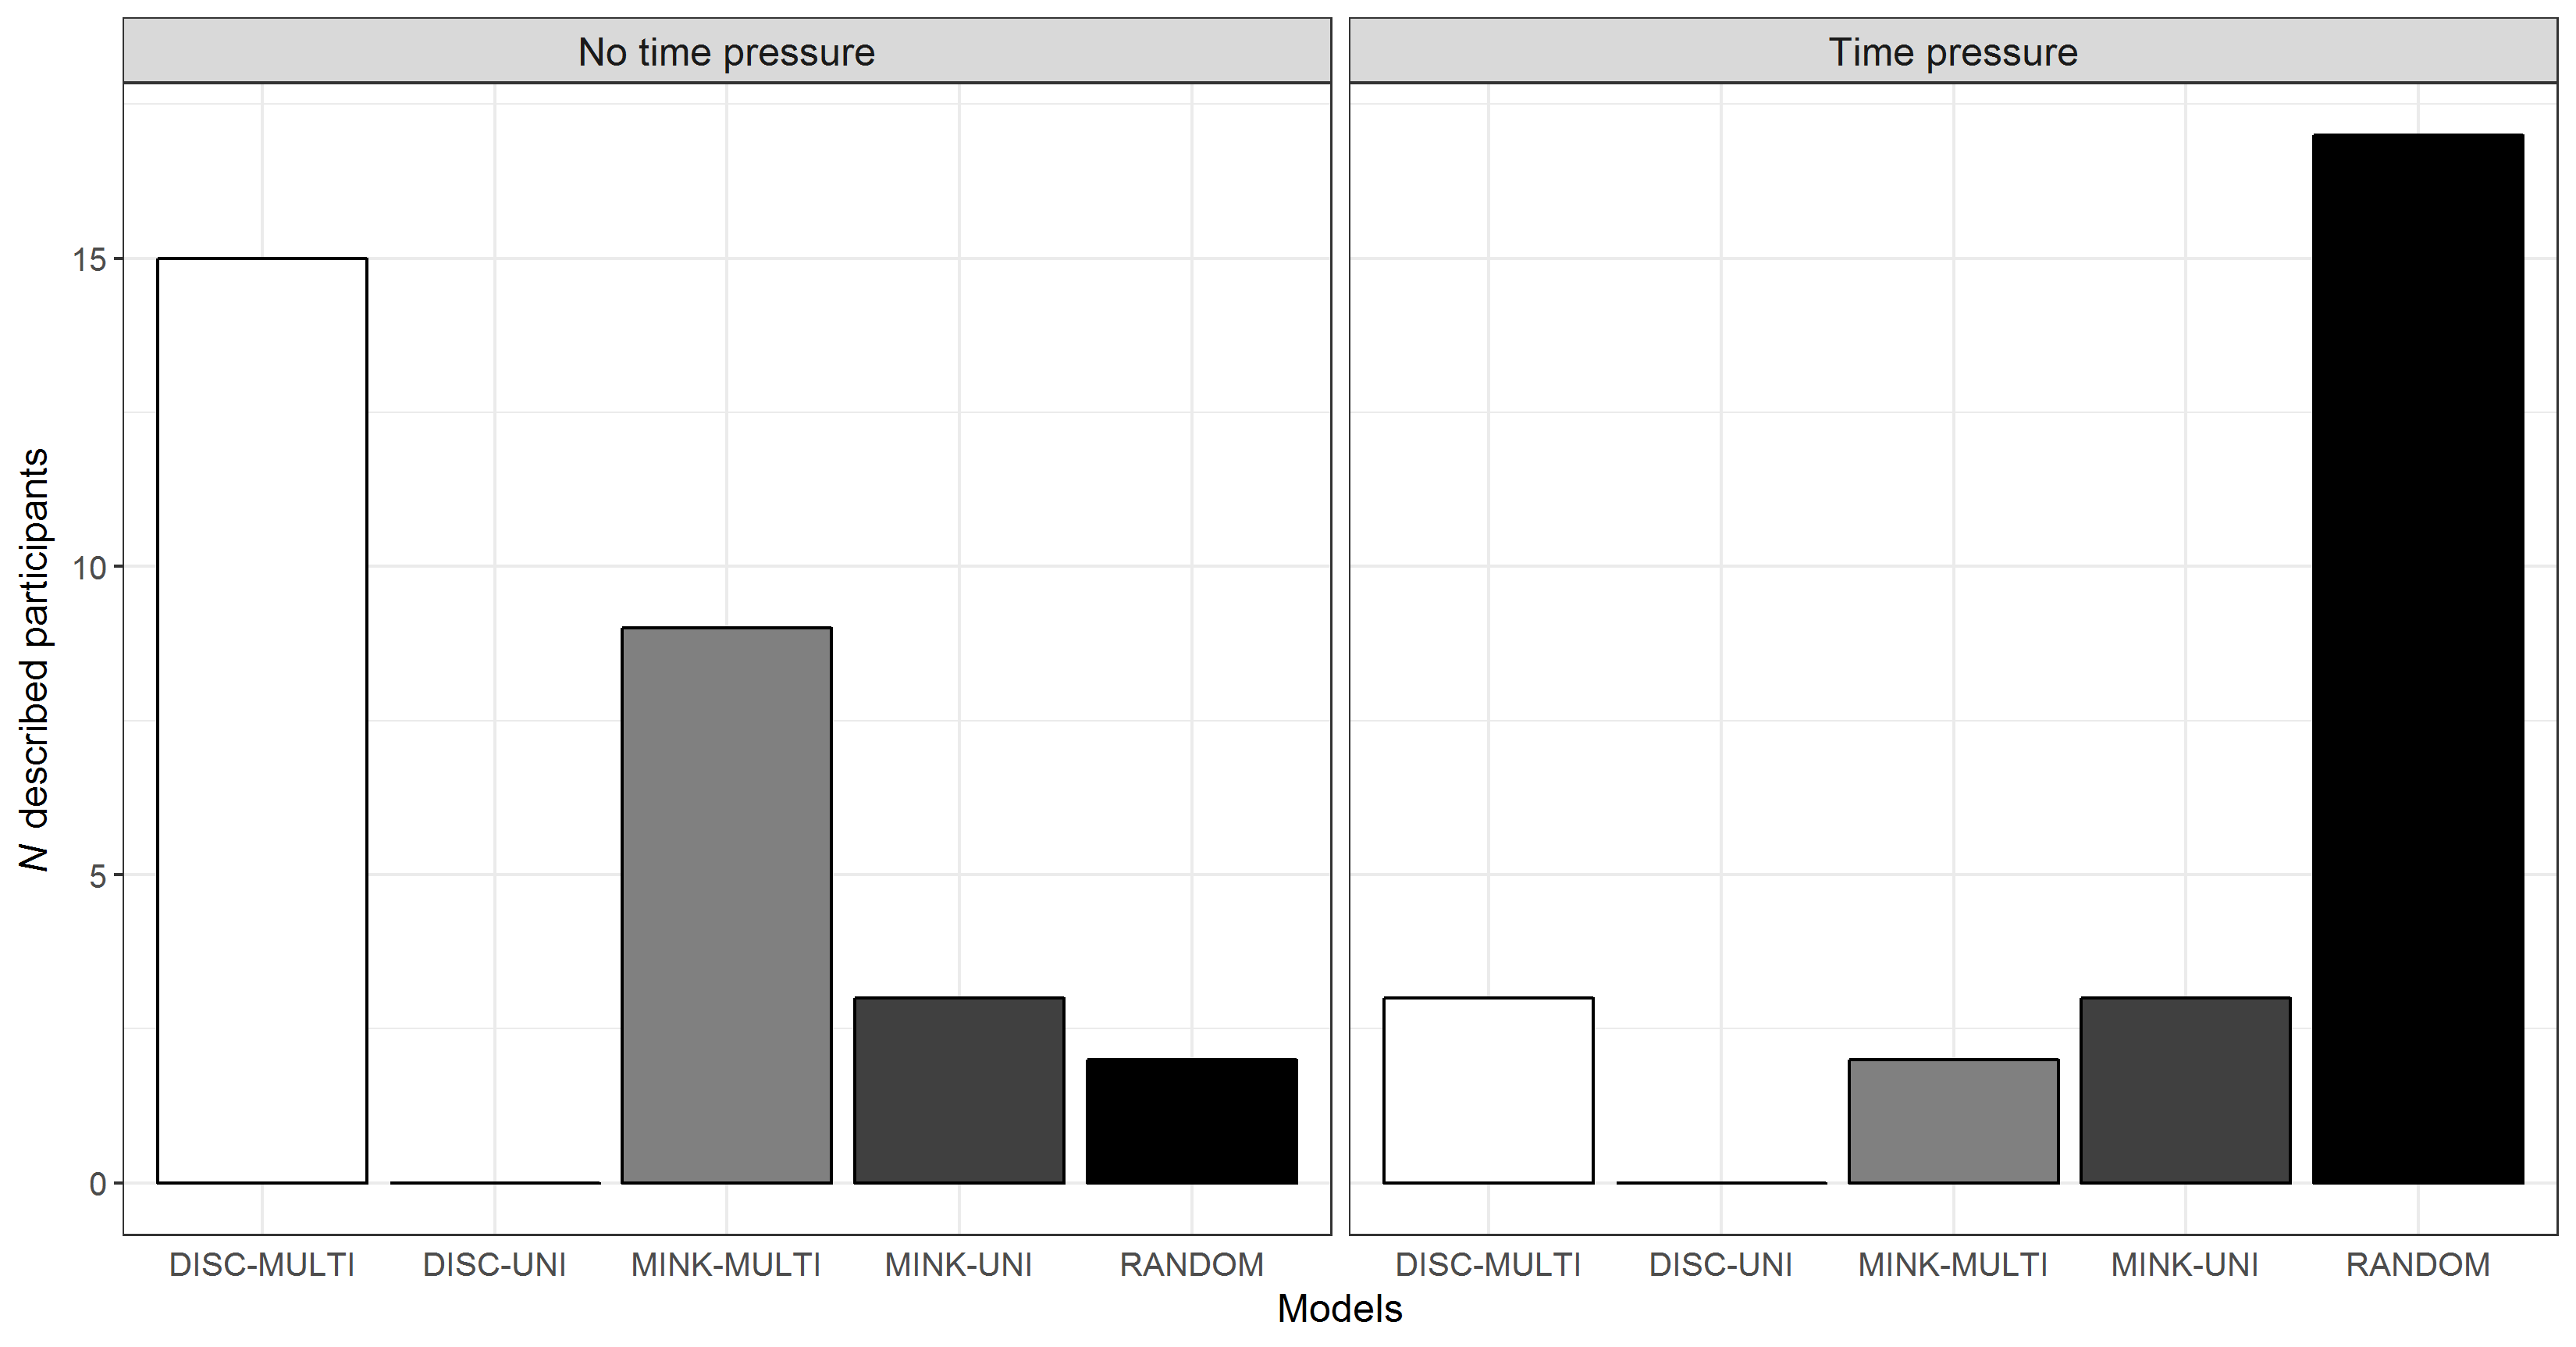
\includegraphics[width = \textwidth]{fig_model_selection.png}
\caption{Number of participants best fit by the generalized context model versions separately for both time pressure conditions. DISC and MINK denote the discrete metric and the Minkowski metric, respectively. MULTI and UNI denote multidimensional and unidimensional model versions, respectively. RANDOM = random choice model.}
\label{fig:model_selection}
\end{figure}

\begin{figure}[htbp]
\centering
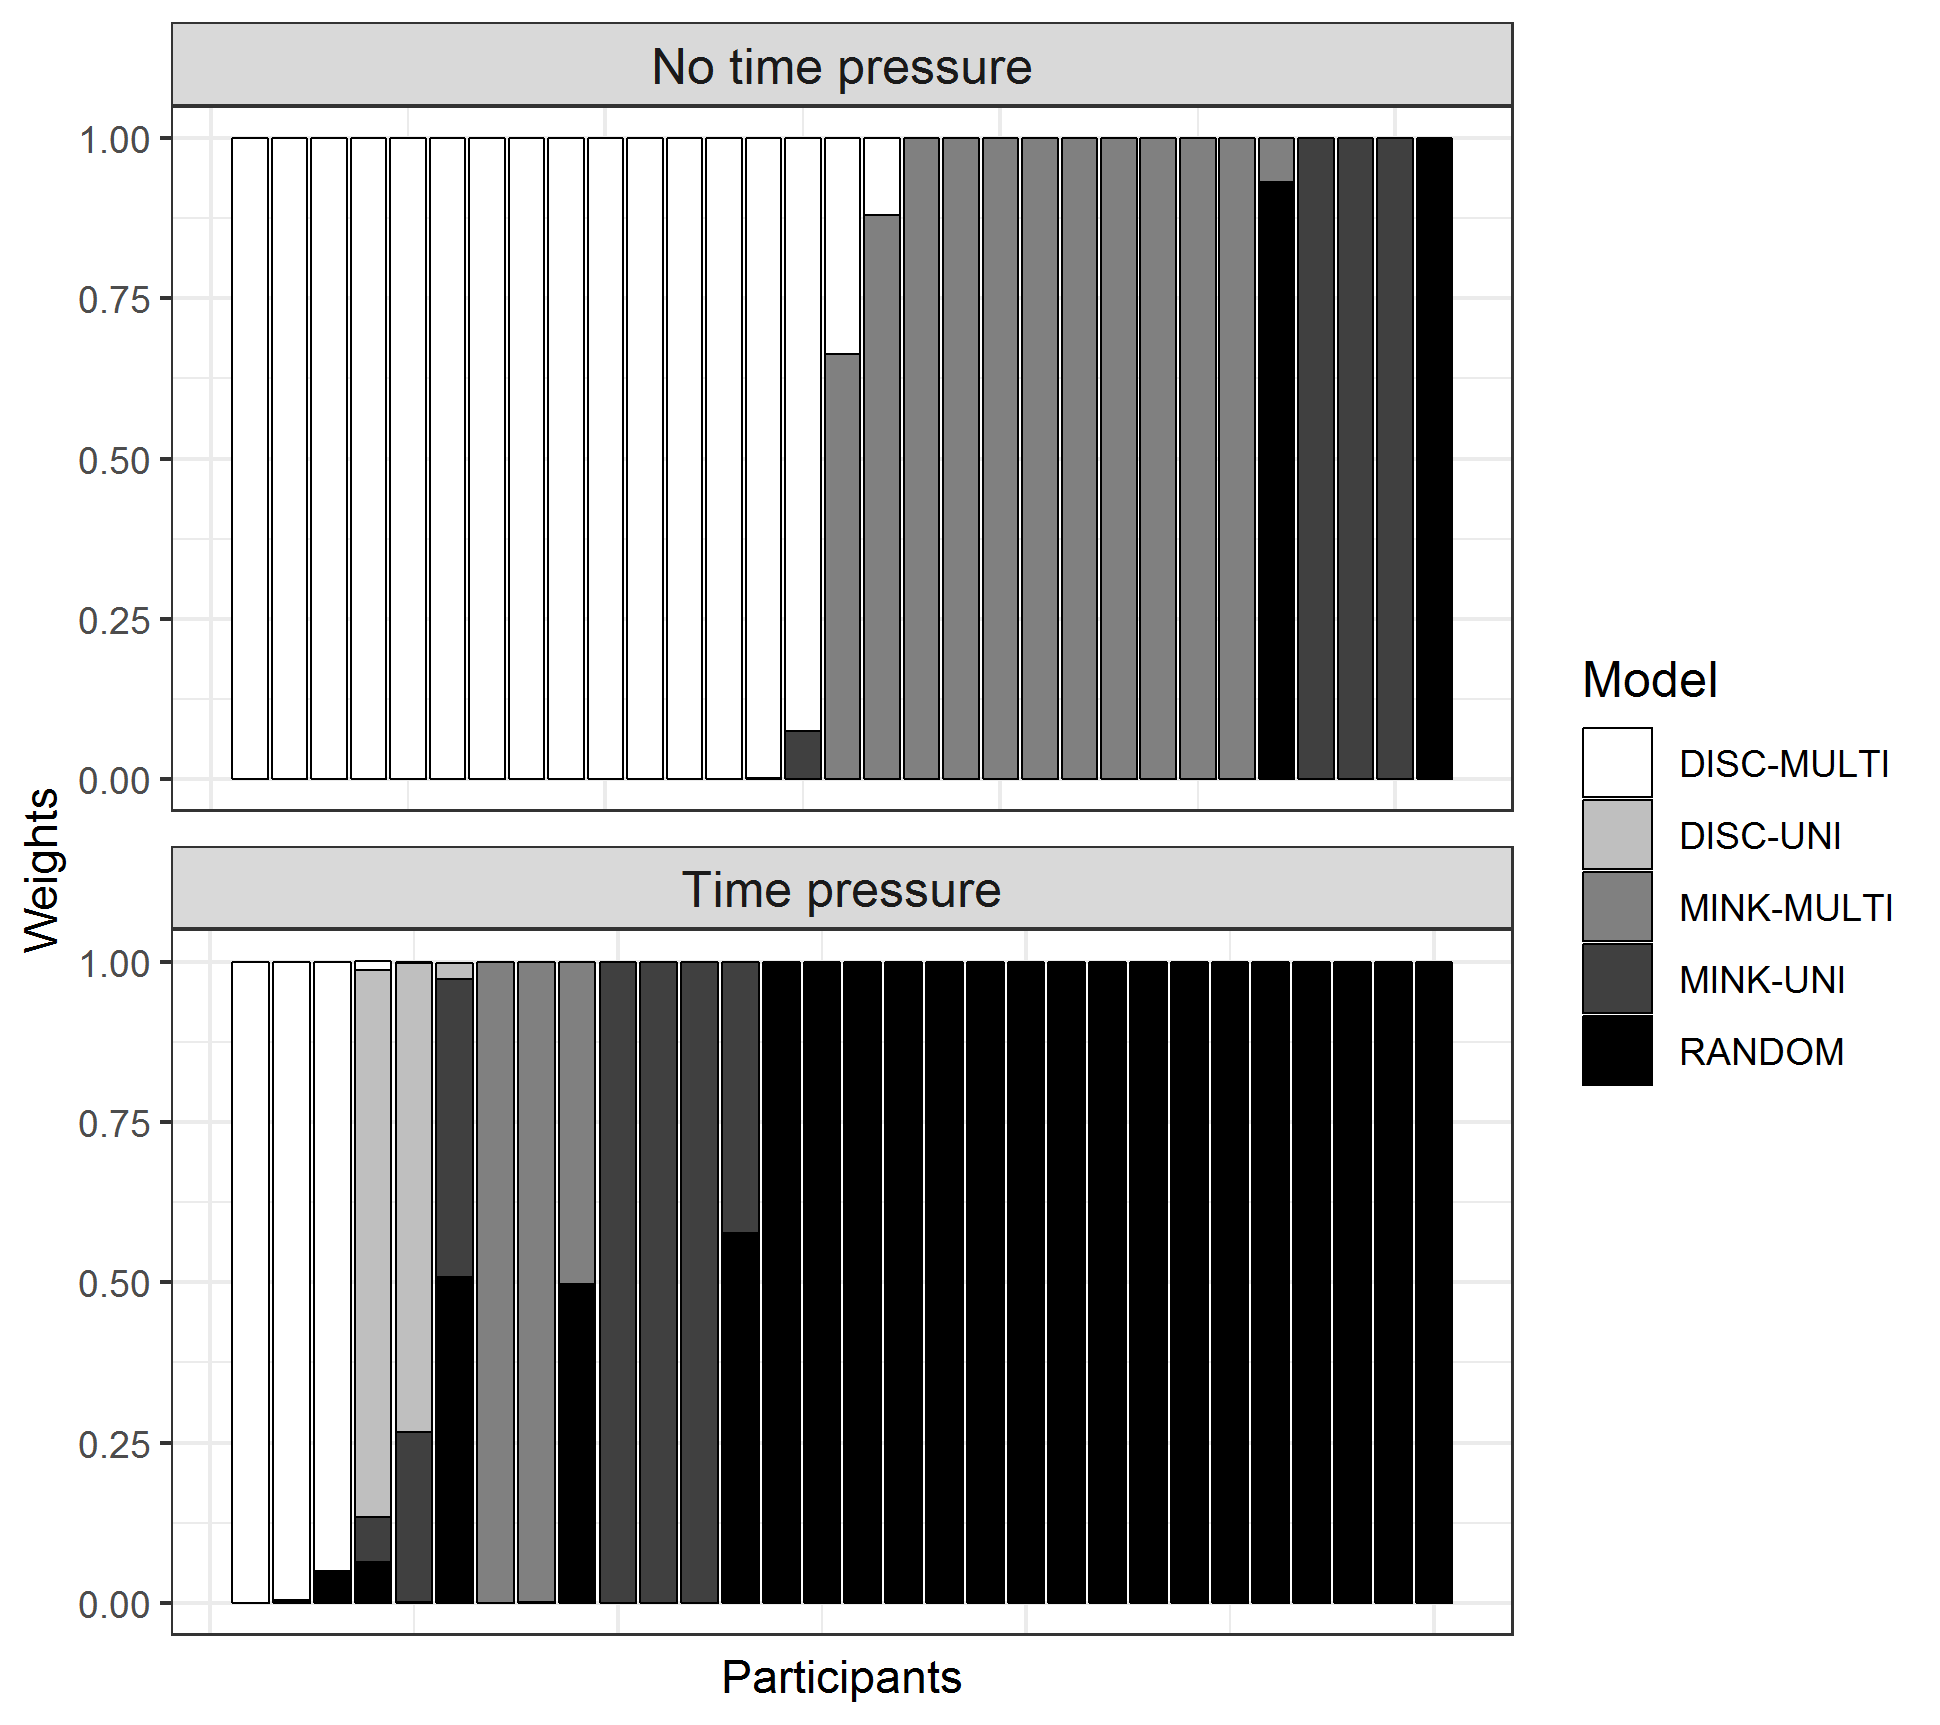
\includegraphics[width = \textwidth]{fig_aic.png}
\caption{Akaike weights of the models for each participant. Each bar represents one participant. The Akaike weights of the different models are stacked upon each other per participant and always sum up to 1. DISC and MINK denote the discrete metric and the Minkowski metric, respectively. MULTI and UNI denote multidimensional and unidimensional model versions, respectively. RANDOM = random choice model.}
\label{fig:aic}
\end{figure}

With time pressure 17 participants were described by the random choice model, three were described by the multidimensional discrete metric and the unidimensional Minkowski metric, respectively, two were described by the multidimensional Minkowski metric, none was described by the unidimensional discrete metric, and five couldn't be described by any model. This observed distribution significantly differed from an expected equal distribution across models ($\chi^{2}(4)$ = 37.2, $p$ < .001). However, H1e (the multidimensional or unidimensional discrete model describes more people than any other model) was rejected, as the random choice model described far more people than any model using the discrete metric (Holm--Bonferroni corrected $p$ = .99). 

Without time pressure 15 participants were described by the multidimensional discrete metric, nine by the multidimensional Minkowski metric, three by the unidimensional Minkowski metric, two by the random choice model, none by the unidimensional discrete model, and two couldn't be described by any model. As in the time pressure condition, this observed distribution significantly differed from an expected equal distribution across models ($\chi^{2}(4)$ = 26.0, $p$ < .001). However, also H2c (the multidimensional Minkowski metric describes more people than any other model) was rejected, as the multidimensional discrete metric described six people more than the multidimensional Minkowski metric (Holm--Bonferroni corrected $p$ = 1).

The rank order of models was defined by the same pairwise comparison procedure using evidence ratios and the same acceptance and rejection criteria as described in the section ''\nameref{sec:res_agg}'' \citep[see also][p. 194]{wagenmakers2004aic}. Using the data with time pressure, the in H1f hypothesized rank order of models (the multidimensional and unidimensional discrete model on the first rank, the unidimensional Minkowski model on the second rank, the multidimensional Minkowski model on the third rank, and the random choice model on the final rank) couldn't be established. Rather, the random choice model outperformed the remaining models, followed by the unidimensional Minkowski model on the second rank, the multidimensional discrete model on the third rank, the unidimensional discrete metric on the forth rank, and the multidimensional Minkowski model on the final rank. Similarly, using the data without time pressure, the in H2c hypothesized rank order of models (the multidimensional Minkowski model describes more people than any other model and the random choice model describes less people than any other model) couldn't be demonstrated. Rather, the multidimensional discrete model outperformed the remaining models, followed by the multidimensional Minkowski model on the second rank, the unidimensional Minkowski model on the third rank, the random choice model on the forth rank, and the unidimensional discrete model on the final rank. 

Finally, the equality of the distribution of the best--predicting models over participants between the conditions with time pressure and without time pressure was found significant using a Fisher's Exact Test ($p$ < .001). Pairwise post hoc comparisons (Holm-Bonferroni-corrected) yielded that H3a (the number of persons described by the multidimensional discrete model is higher in the condition with time pressure than without time pressure) had to be rejected, given that the discrete model described more people without pressure than with time pressure (15 and 3, respectively, \textit{p} = 1). Also, H3b (the number of persons described by the multidimensional Minkowski model is higher in the condition without time pressure than with time pressure) was rejected even though the multidimensional Minkowski model described nine people without time pressure, but only two people with time pressure ($p$ = .08).

\subsection{Explorative Analyses}

\subsubsection{Linear rule--based model}
A linear rule--based model was fit to the test phase data at the participant level, by means of a linear regression with features as predictors. As the test phase included 140 trials per participant, the complete test phase data was fitted and predicted by the regression model in favor of a large data set to fit but also risking over--fitting. In prediction, the fitted regression coefficients for every participants were used. Across participants, the mean estimated regression coefficients (with standard deviations in brackets) were -0.05 (0.18) for the first feature, 0.05 (0.11) for the second feature, -0.18 (0.14) for the third feature, and 0.73 (0.27) for the intercept which represents the stimulus 000. The mean $R^2$ across all participants was .29 (SD = .19).

The linear rule--based model was compared to the other models using the model classification procedure by evidence weights detailed in the section ''\nameref{sec:res_ind}.'' In the condition with time pressure, 28 people were described by the rule--based model, one person by the unidimensional Minkowski model, and one person couldn't be described by any of the models. In the condition without time pressure, 10 people were described by the linear model, eight by the multidimensional discrete model, seven by the multidimensional Minkowski model, and six couldn't be described by any of the models. Across both time pressure conditions, the linear rule--based model was thus the model that could describe the highest number of participants---however, the fact that the same data were used for fitting and predicting potentially overestimates the predictive capacity of the linear regression model. 

\subsubsection{Discrete--threshold metric}
A superordinate version of the discrete metric (i.e., the discrete--threshold metric) was implemented to further test whether people change the distance metric in categorization under time pressure. According to the discrete--threshold metric two features have a distance of 0 if they differ by maximally $\gamma$ and 1 otherwise with the threshold $\gamma$ being a free parameter of the model. In this particular case with four--valued features, $\gamma$ could take the values 0, 1, and 2. If $\gamma$ equals 0, the discrete-threshold metric corresponds to the discrete metric mentioned above. Formally, the discrete--threshold metric is defined as

\begin{equation}
\rho_{m}(x_{im}, x_{jm}) = 
\begin{cases}
	1 & \mid x_{im} - x_{jm} \mid > \gamma \\
	0 & else 
\end{cases},
\end{equation}

where $\rho_{m}(x_{im}, x_{jm})$ is the distance function that checks whether probe $i$ and exemplar $j$ differ by maximally $\gamma$ on dimension $m$. The reminder of the discrete--threshold model is given by equations \ref{eq:probability}, \ref{eq:similarity}, and \ref{eq:distance}. 

As the rule--based model, the discrete--threshold model was fit to the test phase data on the participant level. Learning phase data couldn't be fit, as the stimuli during learning diverged on each feature my maximally 1 rendering the estimation of $\gamma$ impossible. Optimal parameters for each participant were used to compute model predictions and log likelihoods of the same test phase data which was used during fitting. Of all 61 participants, the discrete--threshold model fit 44 (72.13\%) best with $\gamma$ = 0 (which corresponds to the model with the discrete metric), 12 (19.67\%) best with $\gamma$ = 1, and 5 (8.20\%) best with $\gamma$ = 2 with no significant differences between the time pressure conditions ($p$ = .37). In order to reduce the bias caused by fitting to and predicting the same data set, the model comparison analysis retook for all 44 participants best fit by the discrete--threshold model with $\gamma$ = 0 the log likelihood from the equivalent model with the discrete metric that was fit to the learning phase. Given that the majority of participants were best fit by the discrete--threshold model with $\gamma$ = 0, the results of the following model comparison analysis are less affected by over--fitting, although caution is still advisable when interpreting the results. As the discrete--threshold model is a generalization of the generalized context model with the discrete metric, model comparison didn't include the latter model. 

On the aggregate level, using the procedure detailed in ''\nameref{sec:res_agg}'', the discrete--threshold model outperformed the remaining models in the condition without time pressure ($M(LL)$ = -79.09, $Md(LL)$ = -77.14, $SD(LL)$ = 25.50, $MAPE$ = 0.37, $argmax$ = .63, $MSE$ = 0.19).
%, followed by the multidimensional Minkowski model on the second rank, the random--choice model on the third rank, the unidimensional Minkowski model on the forth rank, and the unidimensional discrete model on the final rank. 
With time pressure, the discrete--threshold model scored on the second rank ($M(LL)$ = -101.78, $Md(LL)$ = -96.12, $SD(LL)$ = 28.54, $MAPE$ = 0.45, $argmax$ = .46, $MSE$ = 0.27) and was still outperformed by the random choice model. The rank order of the remaining models is the same as presented in ''\nameref{sec:res_agg}'' and model fit coefficients for the remaining models are shown in Table \ref{tab:fitmeasures}. 
% random, discrete--threshold, MMM, UDM = UMM

On the individual level, using the procedure detailed in ''\nameref{sec:res_ind}'', in the condition without time pressure 14 people were best described by the discrete--threshold model, 10 by the multidimensional Minkowski model, four by the unidimensional Minkowski model, two by the random choice model, and one person couldn't be described by any of the models. In the condition with time pressure 11 people were best described by the random choice model, nine by the discrete--threshold model, three by the unidimensional Minkowski model, and seven couldn't be described by any of the models.

\section{Discussion}
The present thesis examined in a categorization task whether people, given they use the generalized context model \citep{nosofsky1986attention}, apply the heuristic discrete metric instead of the finer--grained Minkowski metric when put under time pressure. Evidence from inferential statistics was not in line with this hypothesis as both with time pressure and without time pressure a cognitive model using the well--established Minkowski metric performed best at predicting participants' behavior. Cognitive modeling, in contrast, yielded that across participants the multidimensional discrete metric outperformed the multidimensional Minkowski metric in both time pressure conditions. Contrary to expectations, the multidimensional discrete metric was the best performing model in the condition without time pressure, but was outperformed by a random choice model in the condition with time pressure---a finding which was corroborated on the participant level. Relative to the condition with time pressure, participants without time pressure used the discrete metric more often and tended to use the multidimensional Minkowski metric as well more often although the latter difference did not reach significance. In sum, these findings do not support the use of the discrete metric under time pressure but indicates that people respond rather using the Minkowski metric (inferential tests) or randomly (cognitive modeling). Cognitive modeling, however, showed that the discrete metric competes the Minkowski metric in describing participants in both time pressure conditions concerning the number of participants it described. Different people may thus represent psychological distance differently independent of the time they have for categorization.

\subsection{Implications for theory and research}
The present results indicate that people do not use different distance metrics in conditions with time pressure and without time pressure. Rather, there is an increase of random categorization when people have reduced cognitive capacities due to time pressure. Similar findings stem from the domain of preferential choice, where cognitive load produced by a secondary task increased participants' inconsistency in preferences \citep{olschewski2018taxing, burks2009cognitive}. Thus instead of yielding a preference shift as claimed in previous literature \citep{burks2009cognitive, benjamin2013behavioral, deck2015effect, schulz2014affect}, people behaved more randomly under high cognitive load. \cite{olschewski2018taxing} modeled choice inconsistency with a probit choice model, where the utility of any given option is variable, but people always choose the option with the momentarily highest utility, and the trembling hand error, where the utility of any given option is fixed, but people choose with a certain probability the option with the smaller utility. 

In analogy to the preferential choice domain, choice inconsistency may be integrated into the generalized context model on the response computation level or on the response execution level: On the response computation level, the analogy to the probit choice model is that people with low cognitive capacities assign not consistently the correct category to the retrieved exemplars. Specifically, each exemplar which is compared to the probe is falsely remembered as a member of the opposite category with a certain probability $p$, which leads to a variance in remembered category membership that is mimicking the variability of utility in the preferential choice domain. On the response execution level, the trembling hand model is to some extent mimicked by Luce's choice axiom of the generalized context model which states that people choose the less likely category with a probability equal to the model's predictions for this category. Note that Luce's choice axiom may be extended with a response--scaling parameter which tunes how deterministically responses are rendered \citep{nosofsky2002exemplar, nosofsky2011generalized, ashby1993relations}. One key difference to the trembling hand model, however, is that even in Luce's choice axiom with the response--scaling parameter the choice of the less likely category is not stable within participants, but stimulus--dependent. Specifically, stimuli with categorization predictions far away from random choice are classified less often into the opposite category than stimuli with categorization predictions close to random choice. If one wanted to implement the trembling hand model in the generalized context model, then Luce's choice axiom needs to replaced by the $argmax$ choice rule, according to which people always choose the category with the highest probability of including the probe, and a trembling hand error, which is a participant--wise constant probability of assigning the probe to the less likely category. However, given that Luce's choice axiom accurately predicts participants' choice proportions \citep{nosofsky1987attention, mckinley1995investigations, lamberts2000information}, it is unclear whether this alternative choice rule may outperform Luce's choice axiom. 

In the present study, choice inconsistency was modeled with $softmax$, which makes categorization responses less deterministic with increasing temperature $\tau$. Fitting the test phase data exploratively showed that $\tau$ was higher under time pressure than without time pressure when using the Minkowski metric (with time pressure: $M$ = 0.38, $Md$ = 0.17, $SD$ = 0.45; without time pressure: $M$ = 0.14, $Md$ = 0.10, $SD$ = 0.09; $t$(31.05) = -2.80, $p$ = .004) and when using the discrete metric (with time pressure: $M$ = 0.98, $Md$ = 0.22, $SD$ = 2.48; without time pressure: $M$ = 0.13, $Md$ = 0.10, $SD$ = 0.07; $t$(29.05) = -1.88, $p$ = .03). Thus, independent of the metric used to fit $\tau$, the results support the insight that people respond more inconsistently under time pressure than without time pressure.

Given the increase of inconsistent responses under time pressure and cognitive load, further research should try to identify the exact causes of choice inconsistency in categorization (i.e., whether responses are inconsistently computed or executed), which is debated as well in other psychological domains \citep{blavatskyy2010models}. To that end, experimental design optimization \citep{myung2004model} could reveal which assumptions have to be met such that different models of stochastic choice can be discriminated from each other and which environments maximize discrimination and are thus potential candidates to test stochastic choice models against each other.

\subsection{Alternative cognitive processes: rule--based decision--making}
Parameter estimates in Figure \ref{fig:par_multidim} show that participants in the aggregate attended primarily to the second feature. However, in our design, the second feature alone was uninformative for participants, as both categories were equally distributed across the values of the second feature in the learning phase. Attending to the second feature thus shifts the predictions of the generalized context model to the random choice level of .50 (see also Table \ref{tab:environment}). While a random choice model or the, in our case, equivalent unidimensional generalized context model attending to the second dimension cannot achieve the accuracy criterion, a sequential rule--based model could potentially explain these results. In fact, the second feature is only uninformative for geometric distance functions, however the value on the second feature can be exploited to decide which of the remaining features should be attended to in a next step. Specifically, given a value of 0 on the second feature, the third dimension discriminates the categories perfectly, and given a value of 1 on the second feature, the first dimension discriminates the categories perfectly. Instead of retrieving exemplars, participants could thus have learned the category structure by using a two--step rule--based model, where the first step is to always attend to the second feature and the second step is to attend to one of the remaining features contingent on the result from the first step.

Literature suggests that people use rules predominantly for well--defined categories \citep{restle1962selection, tom1968attention}, when the stimuli are confusable \citep{rouder2006comparing}, at the beginning of the categorization process \citep{rouder2006comparing}, and conjointly with an exemplar--based strategy such as in ATRIUM \citep{erickson1998rules} and in COVIS \citep{ashby2011covis}. While the categories in the present study were well--defined and the models were fit to the first phase of the experiment, the stimuli were deemed to be discriminable rather than confusable, as feature values were indicated with colored unit squares. Potentially, however, as all features were identical except for the color of the squares, participants may have confused learning stimuli with equal feature values but differently distributed across the features. The insights from past research do thus not disagree with the use of a rule model in the present study. Furthermore the data of the test phase indicate that people without time pressure might have also used a rule to classify the novel stimuli as their responses were very deterministic in comparison to the participants with time pressure. Specifically, the variability of responses by stimulus and participant was higher for the participants with time pressure ($M$ = 0.16, $Md$ = 0.18, $SD$ = 0.09) than for the participants without time pressure ($M$ = 0.06, $Md$ = 0.00, $SD$ = 0.08). Possibly, participants without time pressure generalized the rule with which they learned the category structure in the learning phase to the novel stimuli from the test phase, whereas participants with time pressure lacked the temporal resources to execute the rule and behaved more randomly.

\subsection{Generalization to unfamiliar feature values}
The present results from the test phase further indicate that people might respond differently to novel stimuli with a higher or lower number of familiar feature values. Specifically, the two novel stimuli with two familiar feature values out of three were classified predominantly in line with the multidimensional Minkowski metric version of the generalized context model, whereas the four novel stimuli with one familiar feature value out of three were classified at least partially in line with the multidimensional discrete metric version of the generalized context model. Whereas this raises the possibility that people simplify their distance computation by using the discrete metric when facing novel stimuli with many unfamiliar feature values, past literature on generalization doesn't support this hypothesis, since the predictions of the discrete metric go into the opposite direction of the observed responses \citep{erickson2002rule, denton2008rule}.

In contrast, an extension of the rule--based model outlined above might account for why some novel stimuli of the test phase match the predictions of the multidimensional Minkowski metric, whereas others match the predictions of the multidimensional discrete metric: The rule--based model could first check whether the stimulus has a familiar value on the second feature. If so (i.e., for the stimuli 100 and 003), the model continues with the same two steps as mentioned above. If not (i.e., for the stimuli 221, 231, 321, and 331), the model checks whether one of the remaining features has a familiar value, which in this case would always be the third feature. Given that more members of category A have the same value on the third feature as the stimuli 221, 231, 321, and 331, the model may predict to classify them into category A. 

\subsection{Limitations}
Still needs to be done.

between subjects design --> does one person use the same metric with / without time pressure

stimulus material is a very hard test for the discrete metric

\subsection{Conclusion}
The present study analyzed whether people simplify the categorization process under time pressure by using the generalized context model \citep{nosofsky1986attention} with the heuristic discrete metric instead of the Minkowski metric. Results indicate that people don't change the distance function in dependence of the time available for categorization: Inferential statistics found that the Minkowski model version could predict responses for the test phase both with and without time pressure. Cognitive modeling found that the introduction of time pressure led to an increase of random categorization, which is in line with research on the effects of cognitive load on choice inconsistency \citep{olschewski2018taxing}. These results suggest that people don't adapt their strategy to the available cognitive capacities, but rather display cognitive overload which is manifested by choice inconsistency. Further categorization research may implement different existing models of stochastic choice \citep{blavatskyy2010models, becker1963stochastic} to analyze whether randomness under low cognitive capacities result from inconsistent response computation or execution.

\bibliography{example}

\end{document}

% KLEINSCHREIBUNG von Modellen (z.B. generalized context model anstatt Generalized Context Model)
% Questions: do I have to use the template? nope, should be okay, Jana checks this
% Use Wilcoxon sign test to check whether observed rank orders differ from hypothesized ones? nope
% Table: Do differences between MAPE and M(LL) make sense? could make sense as MAPE is severe when predictions and obs are small
% MINK-MULTI or MMM or GCM with blabla in figures, tables etc.? spell it out!
% check threshold model. what about chisq.multcomp? what about fisher.bintest? Ask again about regression model (half data). 
% Write discrete metric as formula? yes, perhaps begin with degree of belief (evidence strength) = probability for category 1, choice rule and go to distance computation; softmax am Ende der Modellierung --> for both model versions we use the soft max
% Discrete-threshold model fitted to learning phase? 
% without (vs. with) okay? don't use brackets, write with time pressure than without time pressure
% do simulation studies with the MPM have to be in thesis? no

% To do: look for start and end date, which computers were used
% Jäkel, Schölkopf, Wichman: Generalization and similarity 
% search: environment complexity --> metric changes? no feedback --> metric changes? consequences (false categorizations give minus points)
%
% Please see the package documentation for more information
% on the APA6 document class:
%
% http://www.ctan.org/pkg/apa6
%
